%% Chapter 5 — Kubernetes
\setcounter{chapter}{4}
\chapter{Kubernetes}
\chaptersubtitle{서빙 플릿을 움직이는 제어 루프 — 원하는 상태, 정직한 자원 예산, 값비싼 하드웨어를 배치하는 스케줄러}

\begin{calloutbox}{tbbblue}{tbbbluefill}
{\normalsize\bfseries\color{tbbblue}학습 목표}\par\vspace{3pt}
\begin{tbbitemize}
  \item Kubernetes의 핵심 아이디어 하나, 즉 데이터베이스에 원하는 상태를 저장하고 제어 루프로 조정한다는 개념을 설명하고, 파드가 죽거나 노드가 사라지거나 배포가 명세를 바꾸는 등 현실이 원하는 상태에서 벗어날 때 클러스터가 어떻게 움직일지 예측한다.
  \item 컨트롤 플레인과 노드의 구성 요소를 열거하고, 한 번의 \code{kubectl apply}가 API 서버 → etcd → 컨트롤러 → 스케줄러 → kubelet → containerd/runc → 제3장의 네임스페이스와 cgroup으로 이어지는 전 과정을 추적한다.
  \item 모델 서버를 Pod + Deployment + Service로 배포하고, 느린 모델 로딩에 맞춰 시작·준비·활성 프로브를 올바르게 연결하며, 준비 상태가 트래픽과 롤링 업데이트를 어떻게 제어하는지 설명한다.
  \item 리소스 requests와 limits가 실제로 무엇인지, 즉 스케줄러의 산술과 cgroup 파일이라는 차이로 해석하고, 노드 패킹을 직접 계산하며, 서빙 파드에 알맞은 QoS 클래스를 의도적으로 선택한다.
  \item 확장 리소스와 정수 단위 할당, 테인트와 어피니티, 빈 패킹과 분산 배치, 그리고 플릿에서 가장 값비싼 하드웨어를 조용히 놀리는 단편화까지 GPU 스케줄링을 논리적으로 분석한다.
  \item 대표적인 여섯 가지 파드 실패 상태인 Pending, ImagePullBackOff, CrashLoopBackOff, OOMKilled, Evicted, 준비됐지만 라우팅되지 않는 상태(ready-but-unrouted)를 각각의 징후로 진단하고, 상황별로 가장 먼저 실행할 명령을 고른다.
\end{tbbitemize}
\end{calloutbox}

\vspace{5.0pt}

\begin{calloutbox}{tbbteal}{tbbtealfill}
{\normalsize\bfseries\color{tbbteal}핵심 용어}\par\vspace{3pt}
컨트롤 플레인 · API 서버 · etcd · 스케줄러 · 컨트롤러 매니저 · 조정 · kubelet · CRI · 모놀리스 · 마이크로서비스 아키텍처(MSA) · 파드 · pause 컨테이너 · 레이블 / 셀렉터 · Deployment · ReplicaSet · 롤링 업데이트 · Service · ClusterIP / NodePort / LoadBalancer · 엔드포인트 · kube-proxy · CoreDNS · 시작 / 준비 / 활성 프로브 · 요청량(requests) / 상한(limits) · 할당 가능 용량 · 오버커밋 · QoS 클래스 (Guaranteed / Burstable / BestEffort) · 노드 압박 퇴거 · 테인트 / 톨러레이션 · nodeSelector / 어피니티 · 확장 리소스 · nvidia.com/gpu · 디바이스 플러그인 · Pending · CrashLoopBackOff · OOMKilled · Evicted
\end{calloutbox}

\vspace{5.0pt}

\begin{calloutbox}{tbblightgray}{tbbboxfill}
{\normalsize\bfseries\color{tbbink}장 구성}\par\vspace{3pt}
\textbf{5.1} 제어 루프로서의 클러스터    \textbf{5.2} 구조: 자기주장이 있는 데이터베이스    \textbf{5.3} Pods, Deployments, Services — 서빙의 세 축    \textbf{5.4} requests, limits, QoS: 플릿 규모로 확장한 제3장    \textbf{5.5} GPU와 스케줄러    \textbf{5.6} 죽어 가는 파드 현장 안내서    \textbf{5.7} 실습: 모델 서버 오케스트레이션 — 이어서 요약, 연습문제, 더 읽을거리.
\end{calloutbox}

\vspace{3.0pt}

\begin{calloutbox}{tbbamber}{tbbamberfill}
{\normalsize\bfseries\color{tbbamberdark}이 장을 읽는 방법}\par\vspace{3pt}
제3장과 마찬가지로 이 장은 \textbf{터미널을 옆에 두고 읽도록} 썼다. GPU 예시만 관리형 GPU 노드 풀에서 실행했을 뿐, 나머지 모든 터미널 기록은 노트북 클러스터에서 그대로 재현할 수 있다. 유일한 사전 준비는 \code{minikube start}(또는 kind)이며, GPU에서도 명령은 같고 하드웨어만 다르다. YAML 파일은 강의 저장소에 있지만, 한 번 직접 입력해 보는 편이 복제만 하는 것보다 훨씬 유익하다.
\end{calloutbox}

\section{제어 루프로서의 클러스터}

제4장은 만족스러운 결과물로 끝났다. 모델 서버를 이미지로 패키징해 레지스트리에 푸시했고, GPU 접근 방식도 디바이스 플러그인까지 이해했다. VM 한 대에서 \code{docker run} 한 번이면 서빙이 시작된다. 데모라면 이야기는 여기서 끝이다. 그러나 제1장의 실제 요구사항이 한꺼번에 밀려온다. 처리량을 높이고 한 번의 장애가 전체 중단으로 번지지 않게 하려면 \textbf{많은 레플리카}가 필요하다. \textbf{요청을 하나도 놓치지 않는 배포}도 필요하다(제3장의 SIGTERM 이야기가 이제 매주 되풀이된다). 사람이 깨어 있지 않은 \textbf{새벽 3시에 노드가 죽어도} 견뎌야 한다. 하드웨어 요구사항이 서로 다른 \textbf{20개 모델}을 하나의 비용 항목 아래에서 운영해야 한다. 그리고 그 비용에서 가장 큰 몫을 차지하는 GPU가 단지 누군가 작업 배치를 잊었다는 이유로 놀아서는 안 된다.

이 모든 일을 스크립트로 처리할 수도 있다. 2014년 무렵에는 모두가 그랬다. SSH를 순회하는 bash 루프, 헬스 엔드포인트에 curl을 보내 실패한 프로세스를 재시작하는 cron 작업, 어느 모델이 어디서 실행되는지 적어 둔 위키 페이지가 있었다. 이런 스크립트를 현실의 요구에 맞춰 키우다 보면 결국 한 형태로 수렴한다. \textbf{무엇이 실행되어야 하는지 기술한 파일, 그 파일과 현재 실행 상태를 비교하는 루프, 둘 사이의 차이를 없애는 동작}이다. Kubernetes는 이 형태를 산업 수준으로 다듬은 시스템이다. Kubernetes가 이를 외부 세계에 공개하기 전, Google의 내부 시스템 Borg는 바로 이 아이디어로 10년간 운영되었다. 이 형태를 이해하면 나머지는 세부사항일 뿐이다.

\subsection*{시스템 전체를 가르쳐 주는 실험}

실행 중인 클러스터에서 시작하자(실습에서는 \code{minikube start}부터 안내한다). 이 클러스터의 Deployment는 모델 서버 레플리카 세 개를 요구한다. 이제 다른 곳이라면 방해 행위로 여길 일을 해 보자. 하나를 죽인 뒤 곧바로 다시 확인한다.

\begin{terminalbox}
\begin{Verbatim}[breaklines=true,breakanywhere=true,fontsize=\small,formatcom=\color{tbbtermfg},codes=\tbbcodeactive]
$ kubectl get pods
NAME                            READY   STATUS    RESTARTS   AGE
model-server-7d4b9c6f5-8xk2p    1/1     Running   0          2d
model-server-7d4b9c6f5-tq9wz    1/1     Running   0          2d
model-server-7d4b9c6f5-zl6vn    1/1     Running   0          2d
$ kubectl delete pod model-server-7d4b9c6f5-zl6vn   # sabotage
pod "model-server-7d4b9c6f5-zl6vn" deleted
$ kubectl get pods
NAME                            READY   STATUS    RESTARTS   AGE
model-server-7d4b9c6f5-8xk2p    1/1     Running   0          2d
model-server-7d4b9c6f5-tq9wz    1/1     Running   0          2d
model-server-7d4b9c6f5-fh5m8    1/1     Running   0          4s
\end{Verbatim}
\end{terminalbox}
\figcaption{터미널 기록 5-1  파드를 삭제하자 4초 뒤 새 파드가 생겼다(새 이름 접미사와 AGE에 주목하자). 누구도 재시작하지 않았다. 컨트롤러가 2와 3이 다르다는 사실을 알아챘을 뿐이다.}

마지막 줄을 자세히 보자. 이전 파드가 되살아난 것이 아니라, 접미사가 다르고 생성된 지 4초밖에 되지 않은 \textbf{새} 파드다. 아무것도 재시작하지 않았다. 더 정확히 말하면 \textbf{애초에 파드를 요청한 적도 없다.} 단지 명세에 \code{replicas: 3}이라고 적힌 Deployment를 선언했다. 원하는 상태와 실제 상태를 끊임없이 비교하는 루프인 컨트롤러가 2 ≠ 3을 관찰하고 하나를 만들었다. 파드 삭제는 누군가 처리한 이벤트가 아니라 \textbf{편차(drift)}였고, 편차는 교정된다(그림 5-1). 그래서 Kubernetes의 문법은 처음에 낯설다. 동사는 쓰지 않고 \textbf{명사}만 쓴다(객체: "레플리카가 세 개인 Deployment"). 생성, 재시작, 재스케줄링 같은 동사는 명사를 대신해 컨트롤러가 수행하면서 자연스럽게 나타난다.

\begin{tbbfigure}
  \adjustbox{max width=0.94\linewidth,max totalheight=0.46\textheight}{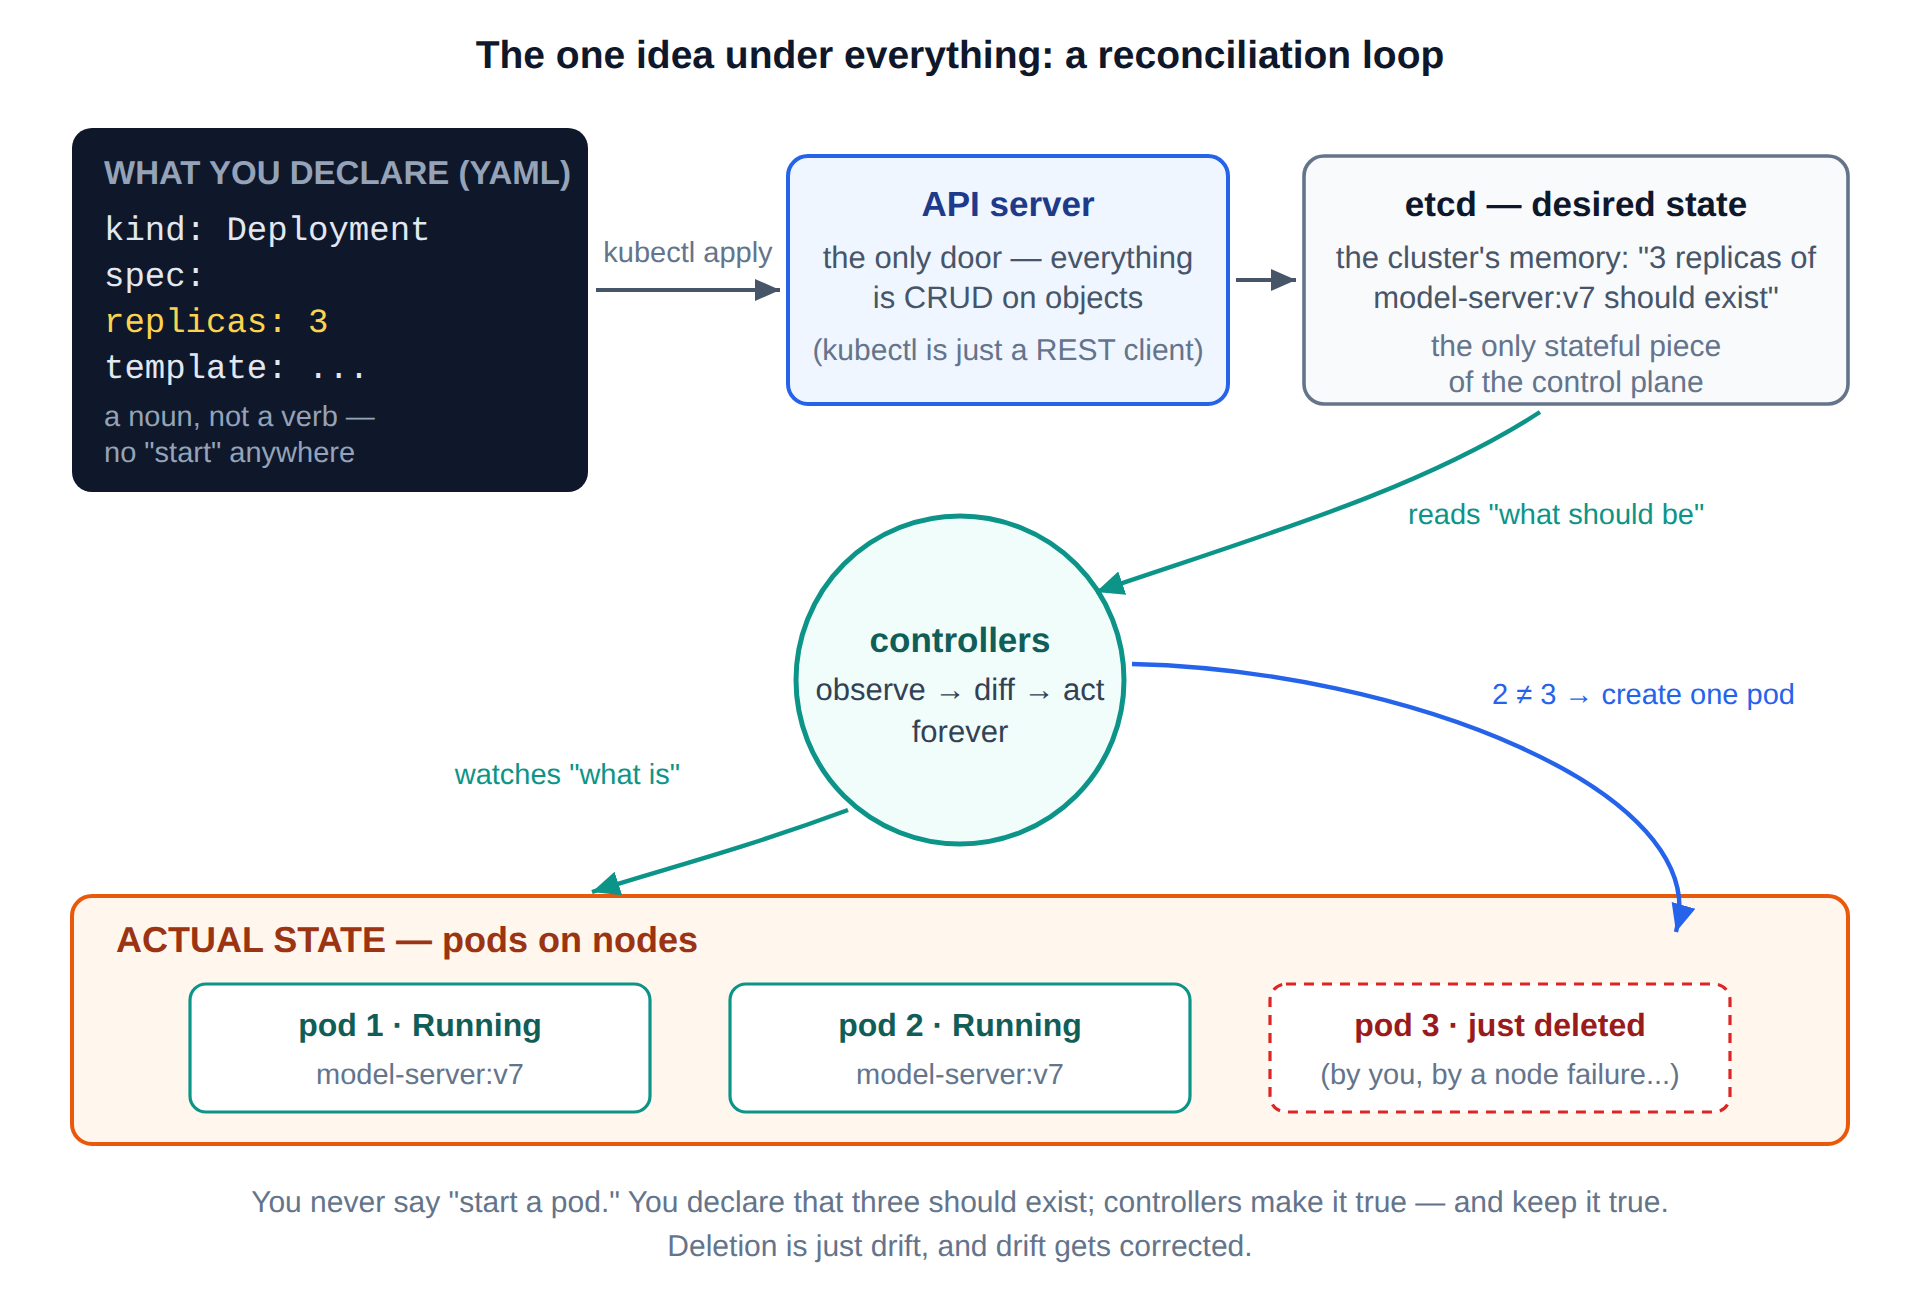
\includegraphics{figures/fig5-1_loop.png}}\\[3pt]
  \figcaption{그림 5-1  조정 루프. 원하는 상태는 API 서버 뒤의 etcd에 저장된다. 컨트롤러는 양쪽을 지켜보며 차이가 사라질 때까지 영원히 동작한다.}
\end{tbbfigure}

\subsection*{새벽 3시에는 선언형이 명령형을 이긴다}

이 차이에는 이름이 있다. \textbf{명령형(imperative)} 시스템은 "서버 세 대를 시작하라" 같은 지시를 받는다. 지시는 한 번 실행되고 나면 시간이 갈수록 효력이 사라진다. 나중에 서버가 죽어도 지시는 이미 끝났으므로, 누군가 이를 발견해 새 지시를 내려야 한다. \textbf{선언형(declarative)} 시스템은 "서버 세 대가 존재한다"라는 \textit{불변 조건}을 유지한다. 불변 조건은 효력을 잃지 않는다. 계속해서 다시 확인하고 강제하므로 "X가 실패하면 어떻게 되는가?"라는 질문의 답은 언제나 같다. \textit{루프가 알아채고 다시 수렴한다.} 가정용 온도조절기도 같은 원리다. 21°C를 선언하면 누군가 창문을 열 때마다 선언을 반복하지 않아도 된다. 서빙 플릿에 꼭 필요한 성질이 바로 이것이다. 새벽 3시의 노드 장애, 실수로 누른 삭제, 플릿을 절반으로 줄여 버린 배포는 루프의 눈에는 모두 똑같은 편차다.

선언형 습관은 이 강의 뒤쪽에서도 복리처럼 이익을 낸다. 12주 차에 오토스케일링을 추가해도 오토스케일러는 전혀 새로운 종류의 장치가 아니다. 부하가 커지면 \code{replicas: 3}을 \code{replicas: 7}로 바꾸고 나머지는 이 절의 루프에 맡기는 \textbf{또 하나의 원하는 상태 작성자}일 뿐이다. 13주 차에 CI/CD로 배포를 자동화할 때도 파이프라인의 마지막 동작은 객체 한 줄을 바꾸는 것이다. 이 강의의 운영 파트에서 일어나는 모든 일은 사람이나 시스템이 명사를 편집하는 과정이며, 유일한 엔진은 그림 5-1의 루프다.

\subsection*{이 장이 실제로 다루는 것}

서빙 엔지니어에게 Kubernetes는 네 가지 높이에서 중요하며, 이 장은 각 층을 차례로 살펴본다. 가장 위의 \textbf{제어 루프}(이 절)는 앞으로 마주칠 모든 실패 상황에서 시스템이 어떻게 움직이는지 설명한다. 한 층 아래의 \textbf{객체}, 즉 Pod, Deployment, Service(§5.3)는 모델 서버를 기술하고 상태를 확인하며 안정적인 주소를 부여하는 어휘다. 그 아래의 \textbf{리소스와 QoS}(§5.4)는 제3장의 cgroup 벽을 플릿 규모로 대신 작성하는 곳이다. 이제 자다가도 설명할 수 있는 OOM 동작도 여기에 포함된다. 가장 아래에서는 \textbf{스케줄러}(§5.5)가 어떤 값비싼 GPU에서 어떤 모델을 실행할지 결정한다. 매달 청구서로 결과가 드러나는 배치 문제다. 마지막으로 §5.6에서는 이 전체 스택을 실제 업무에서 쓰이는 형태, 즉 체계적인 진단법으로 바꾼다.

\begin{calloutbox}{tbbpurple}{tbbpurplefill}
{\normalsize\bfseries\color{tbbpurple}생각해 보기}\par\vspace{3pt}
\begin{tbbitemize}
  \item 컨트롤러는 2 ≠ 3을 보고 파드를 하나 만들었다. 이번에는 ReplicaSet이 선택하는 것과 같은 레이블(label)을 단 네 번째 파드를 직접 만들었다고 하자. 컨트롤러는 무엇을 해야 하며, 이는 구성원 자격을 결정하는 방식에 관해 무엇을 뜻하는가?
  \item 컨트롤러 자체가 중단되었을 때 조정 루프(reconciliation loop)가 다시 복구되는 능력이, 명령형 스크립트를 실행하던 호스트가 중단되었을 때보다 뛰어난 이유는 무엇인가? (힌트: 올바르게 재개하려면 각각 어떤 상태가 필요한가?)
  \item 12주 차에는 Horizontal Pod Autoscaler가 부하에 반응해 한 객체의 정수 하나를 바꾼다. 그 뒤 자동으로 일어나야 한다고 이 절에서 설명한 모든 일을 나열해 보자. 오토스케일러 자체가 알아야 하는 것은 놀라울 만큼 적다.
\end{tbbitemize}
\end{calloutbox}

\section{구조: 자기주장이 있는 데이터베이스}

신비감을 걷어 내면 Kubernetes의 아키텍처는 한 문장으로 정리된다. \textbf{앞에는 API(API 서버)가 있고 뒤에는 수많은 제어 루프(컨트롤러, 스케줄러, 노드마다 하나씩 있는 kubelet)가 붙은 데이터베이스(etcd)}다. 나머지는 모두 부연 설명이다. 그림 5-2는 구성 요소를 한눈에 펼쳐 보인다. 이 절에서는 각 요소를 하나씩 설명한 뒤, 한 번의 \code{kubectl apply}가 모든 요소를 통과하는 과정을 추적한다. 실제로 디버깅하는 대상은 개별 부품이 아니라 이 연결 고리이기 때문이다.

\begin{tbbfigure}
  \adjustbox{max width=0.94\linewidth,max totalheight=0.46\textheight}{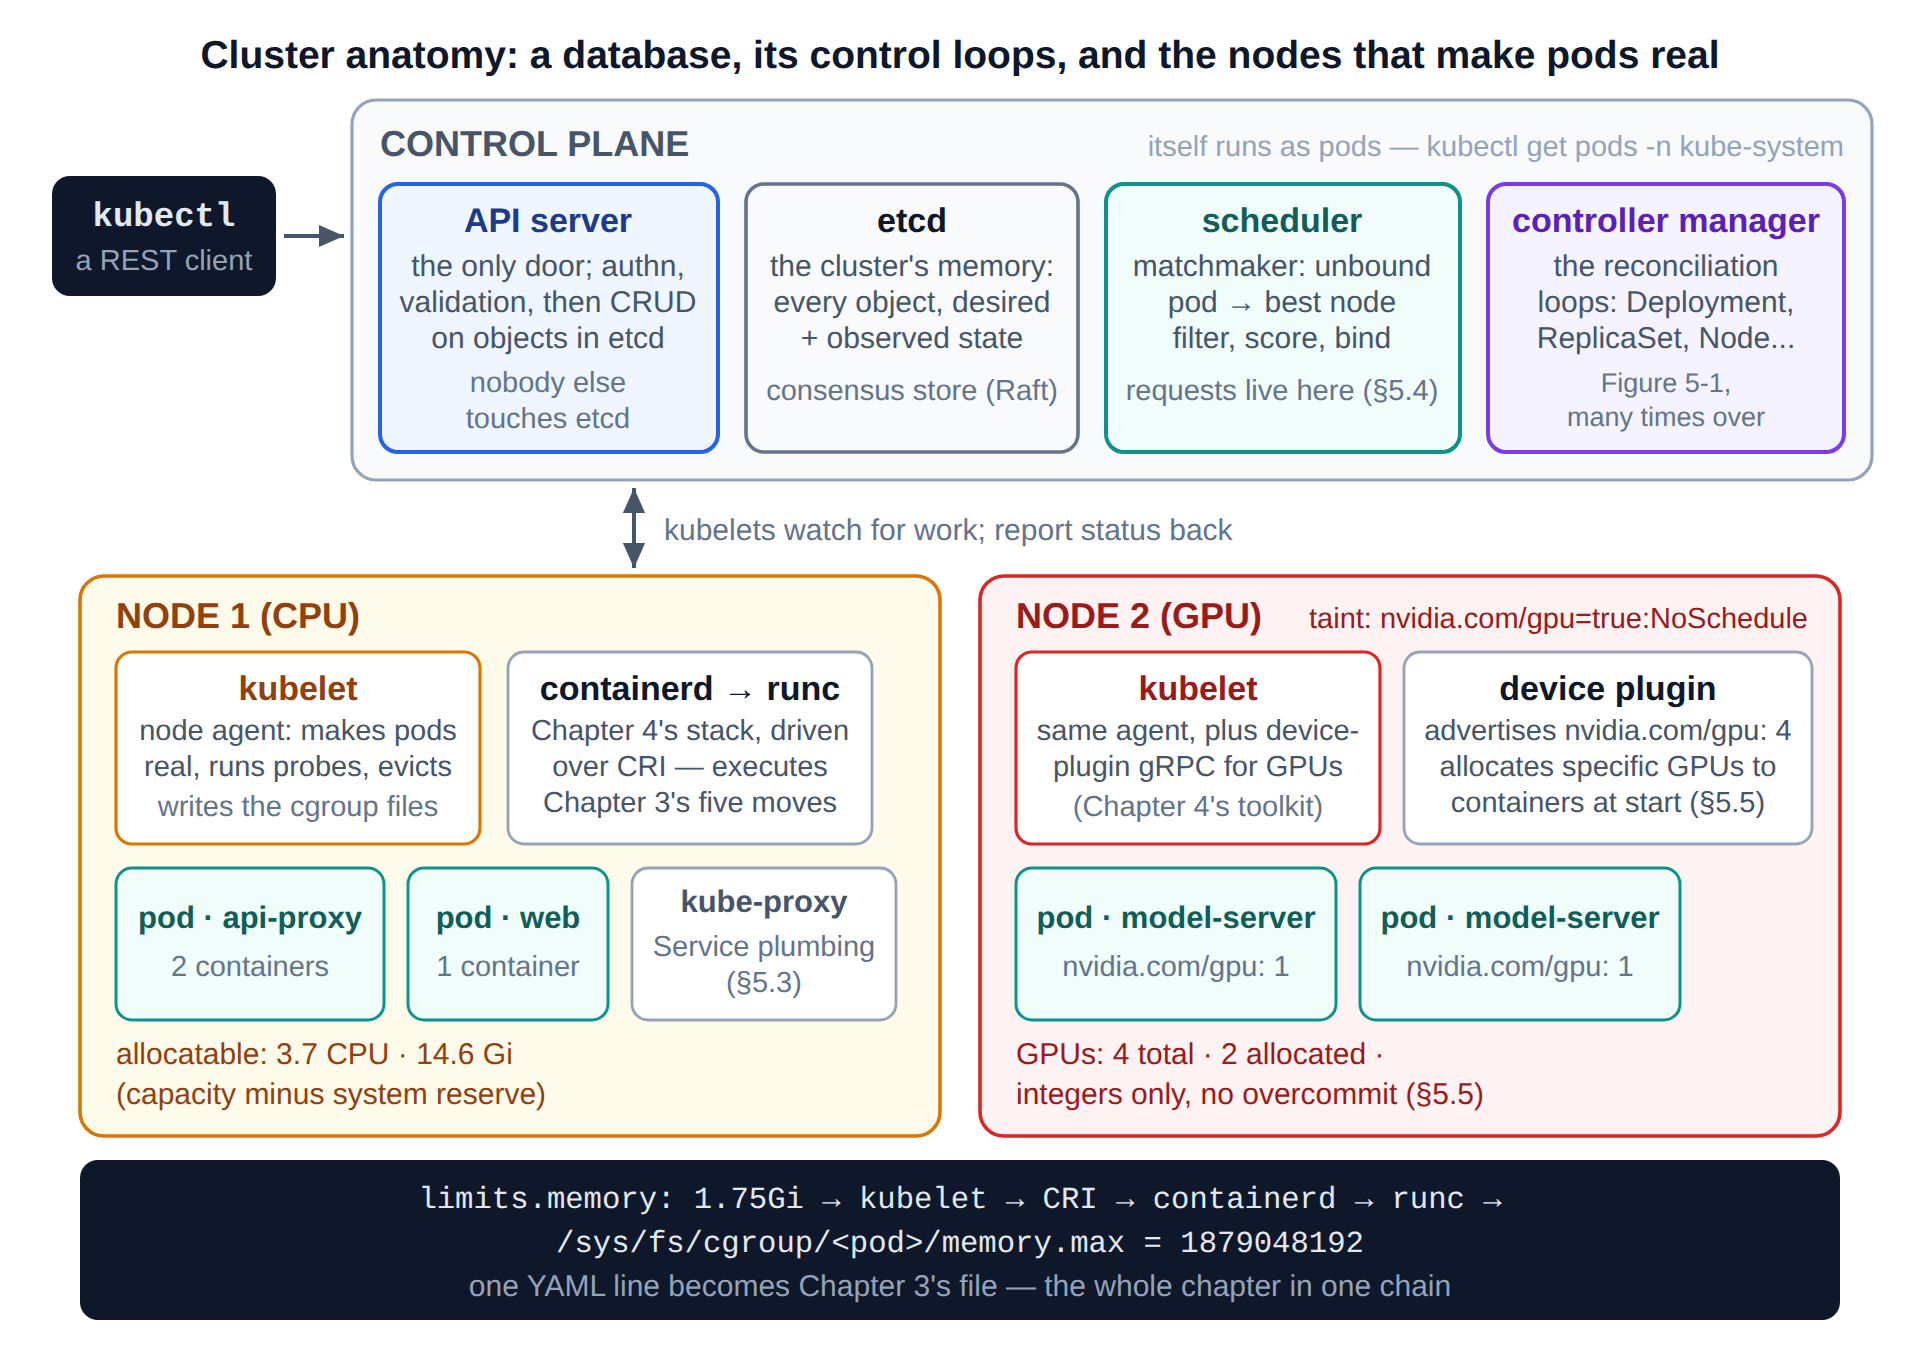
\includegraphics{figures/fig5-2_architecture.png}}\\[3pt]
  \figcaption{그림 5-2  클러스터 구조. 컨트롤 플레인은 원하는 상태를 저장하고 조정한다. 각 노드의 kubelet은 제4장의 런타임 스택을 거쳐 파드를 현실로 만들며, 그 끝에는 제3장의 네임스페이스와 cgroup이 있다.}
\end{tbbfigure}

\subsection*{컨트롤 플레인: 구성 요소별 한 문단}

\textbf{API 서버}는 유일한 출입구다. kubectl을 사용하는 사람, 모든 컨트롤러, 모든 kubelet은 오직 API 서버하고만 통신한다. 그 외에는 아무것도 etcd에 접근할 수 없다. API 서버는 인증하고 권한을 확인하며 유효성을 검사한 뒤, 다소 싱거울 만큼 단순한 일을 한다. 객체에 CRUD를 수행한다. 내부에 숨겨진 오케스트레이션 두뇌는 없다. 출력 상세도를 높이면 \code{kubectl}조차 얇은 REST 클라이언트일 뿐이라는 사실이 드러난다.

\begin{terminalbox}
\begin{Verbatim}[breaklines=true,breakanywhere=true,fontsize=\small,formatcom=\color{tbbtermfg},codes=\tbbcodeactive]
$ kubectl get pods -v=8 2>&1 | grep -E "GET http"
GET https://192.168.49.2:8443/api/v1/namespaces/default/pods?limit=500
# kubectl get pods = one HTTP GET. kubectl is a REST client with manners.
$ kubectl get pods -n kube-system
NAME                               READY   STATUS    RESTARTS      AGE
etcd-minikube                      1/1     Running   0             9d
kube-apiserver-minikube            1/1     Running   0             9d
kube-controller-manager-minikube   1/1     Running   0             9d
kube-scheduler-minikube            1/1     Running   0             9d
coredns-5dd5756b68-mfqpx           1/1     Running   0             9d
kube-proxy-b47rl                   1/1     Running   0             9d
\end{Verbatim}
\end{terminalbox}
\figcaption{터미널 기록 5-2  두 가지 오해를 걷어 낸다. kubectl은 HTTP이며, 컨트롤 플레인 자체도 kube-system 네임스페이스의 파드로 실행된다. 시스템이 자기 자신을 관리하는 셈이다.}

\textbf{etcd}는 클러스터의 기억 장치다. 원하는 상태와 마지막으로 관찰한 상태를 포함한 모든 객체를 보관하는 작고 일관된(Raft 합의 기반) 키-값 저장소다. 이것이 \textit{유일한} 상태 저장 구성 요소다. 다른 구성 요소는 언제든 중단해도 재시작한 뒤 API 서버를 다시 지켜보는 것만으로 작업에 필요한 지식을 복구한다. 잠시 감탄할 만한 설계 결정이다. 상태는 복제된 저장소 하나에 집중하고, 나머지는 모두 상태가 없으며 교체 가능하게 만든다. 나중에 직접 설계할 서빙 시스템에도 똑같이 적용하라고 권할 형태다.

\textbf{스케줄러}는 역할이 매우 좁은 중매자다. 아직 노드가 배정되지 않은 파드를 지켜보다가, 각 파드에 가장 적합한 노드를 고르고(먼저 필터링하고 점수를 매기는 과정은 GPU 때문에 흥미로워지는 §5.5에서 해부한다), 그 선택을 파드 객체에 다시 기록한다. 하는 일은 이것뿐이다. 아무것도 시작하지 않고 어떤 노드도 직접 건드리지 않는다. \textbf{컨트롤러 매니저}는 §5.1의 조정 루프들을 실행한다. Deployment 컨트롤러, ReplicaSet 컨트롤러, 죽은 노드를 알아채는 노드 수명 주기 컨트롤러를 비롯한 수십 개의 루프가 있으며, 각 루프는 한 객체 유형을 대상으로 "관찰하고, 차이를 찾고, 동작하는" 작은 과정이다.

모든 노드에서 \textbf{kubelet}은 손발 역할을 한다. API 서버를 지켜보다가 \textit{자기} 노드에 바인딩된 파드를 현실로 만든다. 제4장의 containerd → runc 스택 앞에 놓인 gRPC 인터페이스인 CRI를 통해 컨테이너 런타임에 지시하고, 볼륨을 마운트하며, §5.3의 프로브를 실행하고, 상태를 다시 보고한다. 메모리 압박이 생기면 §5.4의 퇴거도 수행한다. 이 설명에서 kubelet이 누구인지 눈여겨보자. 바로 \textbf{제3장이 계속 예고했던 대필자}다. 파드가 \code{limits.memory: 1.75Gi}를 선언하면, 런타임을 거쳐 \code{memory.max} 파일에 \code{1879048192}가 나타나게 만드는 주체가 kubelet이다. 그 옆에는 §5.3의 Service NAT를 프로그래밍하는 \textbf{kube-proxy}가 실행된다. GPU 노드에서는 제4장의 \textbf{디바이스 플러그인}도 함께 실행되어 GPU가 몇 개 있고 어느 것이 비어 있는지 kubelet에 알려 준다.

\subsection*{한 번의 apply를 처음부터 끝까지}

이제 연결 고리를 따라가 보자. 레플리카가 세 개인 새 모델 서버를 위해 \code{kubectl apply -f deployment.yaml}을 입력한다. 전체를 지휘하는 주체 없이 다음 일이 순서대로 일어난다.

\begin{tbbitemize}
  \item \textbf{1 — 저장.} API 서버가 Deployment 객체의 유효성을 검사하고 etcd에 기록한다. 아직 아무것도 실행되지 않았다. 데이터베이스의 한 행만 바뀌었다.
  \item \textbf{2 — 확장.} Deployment 컨트롤러는 일치하는 ReplicaSet이 없는 Deployment를 발견하고 하나를 만든다(이번에도 객체다). ReplicaSet 컨트롤러는 원하는 수가 3인데 실제 수가 0임을 알아채고, \code{nodeName}이 비어 있는 Pod 객체 세 개를 만든다.
  \item \textbf{3 — 배치.} 스케줄러는 노드에 바인딩되지 않은 파드 세 개를 발견하고, 파드마다 필터링과 점수 계산을 거쳐 노드 이름을 기록한다. 여전히 어느 곳에서도 아무것도 실행되지 않았다.
  \item \textbf{4 — 실체화.} 선택된 각 노드의 kubelet은 자신에게 바인딩된 파드를 발견한다. 이미지가 없으면 가져오고(제3장에서 계산한 25–60 s의 콜드 풀 시간이 노드마다 적용된다), containerd → runc를 구동해 pause 컨테이너와 서버 컨테이너를 만든다. 분리된 네임스페이스, 작성된 cgroup 파일, 마운트된 overlayfs까지 제3장의 다섯 동작을 시스템이 수행한다.
  \item \textbf{5 — 보고.} kubelet이 상태를 다시 게시하고 프로브가 시작된다. 준비 상태 검사를 통과하면 파드의 IP가 Service 엔드포인트(§5.3)에 들어가고 트래픽이 흐른다.
\end{tbbitemize}

이 연결 고리에서 두 가지는 특히 강조할 가치가 있다. 첫째, \textit{Kubernetes라는 이름의 무언가가 컨테이너를 실행한 것이 아니다.} 실행은 runc가 했고, Kubernetes는 위치를 결정하고 상태를 기록했다. 제3장이 컨테이너의 신비를 걷어 냈다면, 이 절은 오케스트레이터의 신비를 걷어 낸다. 같은 커널 메커니즘 주위에서 장부를 관리할 뿐이다. 둘째, \textit{연결 고리의 모든 화살표는 API 서버에 대한 watch다.} 구성 요소끼리는 서로 호출하지 않는다. 이처럼 철저히 분리했기 때문에 어느 한 구성 요소가 멈춰도 시스템이 견딘다. 작업은 etcd에서 기다리고, 재개한 구성 요소가 가져가면 된다. (또한 컨트롤 플레인에 문제가 생겨도 데이터 플레인이 계속 서빙한다는 뜻이다. 이미 실행 중인 파드, 이미 프로그래밍된 Service 경로, 이미 작성된 cgroup 파일은 계속 동작하는 데 허가가 필요 없다. 컨트롤 플레인이 돌아올 때까지 아무것도 \textit{변경}하지 못할 뿐이다.)

\begin{calloutbox}{tbbpurple}{tbbpurplefill}
{\normalsize\bfseries\color{tbbpurple}생각해 보기}\par\vspace{3pt}
\begin{tbbitemize}
  \item etcd가 10분 동안 쿼럼을 잃었다. 다음 가운데 계속 동작하는 것은 무엇이며, 그 이유는 무엇인가? (a) 기존 파드의 트래픽 서빙, (b) 파드로 향하는 Service 라우팅, (c) 롤링 업데이트, (d) 파드 중단 후 자가 복구
  \item 구성 요소끼리 직접 통신하게 하지 않고(예: 스케줄러 → kubelet) API 서버에 대한 watch를 거치게 한 이유는 무엇인가? 이 간접 계층이 흡수하는 실패 시나리오 두 가지를 들어 보자.
  \item 컨트롤러가 중단되었다가 5분 뒤 재시작했다. 관찰한 상태를 기준으로 동작하는 "레벨 트리거" 조정이 이벤트를 기준으로 동작하는 "에지 트리거" 방식보다 이 상황을 자연스럽게 견디는 이유를 설명하자.
\end{tbbitemize}
\end{calloutbox}

\section{Pods, Deployments, Services — 서빙의 세 축}

이 강의에서 실행할 거의 모든 서빙 워크로드는 세 객체가 떠받친다. \textbf{Pod}는 서버와 보조 컨테이너를 묶는 실행 단위다. \textbf{Deployment}는 개수, 버전, 업그레이드 방식을 관리하는 플릿 관리자다. \textbf{Service}는 언젠가 사라질 레플리카 앞에 하나의 이름을 제공하는 안정적인 주소다. 이 세 가지를 깊이 이해하면 앞으로 만날 Kubernetes YAML 대부분이 그 변형으로 보인다.

\subsection*{먼저 워크로드의 형태부터: 마이크로서비스 개요}

세 객체를 해부하기 전에 이들이 암묵적으로 가정하는 아키텍처 스타일에 이름을 붙여 보자. 전통적인 대안은 \textbf{모놀리스(monolith)}다. UI, 비즈니스 로직, 데이터 접근 같은 모든 기능을 하나의 배포 단위에 담고, 하나의 코드베이스에서 빌드해 하나의 결과물로 출시하며, 전체 복사본을 더 실행해 확장한다. \textbf{마이크로서비스(microservice) 아키텍처(MSA)}는 애플리케이션을 작고 독립적으로 배포 가능한 서비스로 나눈다. 각 서비스는 하나의 기능과 이상적으로는 자체 데이터를 소유하고, HTTP나 gRPC 같은 네트워크 API를 통해서만 다른 서비스에 기능을 제공한다. 보통 전담 팀 아래에서 독자적인 출시 주기로 발전한다.

업계가 유행을 좇아 이 구조로 옮겨 간 것은 아니다. 이점은 운영에서 드러난다. \textbf{독립 배포}: 결제 서비스를 다시 출시하지 않고도 추천 서비스를 매일 배포할 수 있다. \textbf{독립 확장}: 부하가 몰리는 곳에만, ML 시스템이라면 GPU가 필요한 곳에만 레플리카를 추가한다. \textbf{장애 격리}: 추천 서비스가 중단되면 페이지 품질은 낮아져도 결제까지 멈추지는 않는다. \textbf{조직과의 정합성}: 작은 팀이 작은 서비스를 처음부터 끝까지 소유한다. 물론 대가도 분명하며, 이것이 솔직한 나머지 절반이다. 프로세스 내부 함수 호출이 모두 \textbf{네트워크 호출}로 바뀌어 지연 시간, 타임아웃, 부분 실패, 분산 디버깅을 동반한다. 하나의 배포 대상은 \textbf{N개의 배포 대상}이 되고, 각각 빌드, 버전 관리, 서비스 발견(service discovery), 상태 검사, 확장, 모니터링이 필요하다.

\begin{calloutbox}{tbbteal}{tbbtealfill}
{\normalsize\bfseries\color{tbbteal}모놀리스 대 마이크로서비스 — 한눈에 보는 절충 관계}\par\vspace{3pt}
\begin{tbbitemize}
  \item \textbf{배포} — 모놀리스: 결과물 하나를 한 번에 전체 출시. MSA: 서비스마다 독립적인 주기로 출시.
  \item \textbf{확장} — 모놀리스: 전체를 복제. MSA: 부하가 큰 경로만 확장(서빙에서는 GPU를 많이 쓰는 부분만 확장).
  \item \textbf{실패} — 모놀리스: 운명을 공유. MSA: 장애 영향 범위를 격리. 단, 타임아웃과 대체 경로를 실제로 설계해야 하며 저절로 얻어지지는 않는다.
  \item \textbf{호출} — 모놀리스: 프로세스 내부에서 나노초 단위. MSA: 네트워크를 거치므로 지연 시간과 부분 실패가 생기고, 무슨 일이 있었는지 재구성하려면 추적이 필요하다.
  \item \textbf{조직} — 모놀리스: 하나의 코드베이스, 회의로 조율. MSA: 서비스별 팀(Conway의 법칙을 의도적으로 활용).
\end{tbbitemize}

한 문장으로 요약하면 \textbf{코드 복잡성을 운영 복잡성과 맞바꾸며, Kubernetes는 업계가 운영 측면을 표준화한 결과물이다.}
\end{calloutbox}

\vspace{3.0pt}

마지막 문장이 이 장의 존재 이유를 설명한다. MSA가 만드는 운영 부담은 도입 조직마다 거의 같다. 그래서 산업화할 수 있었고, 그 산업화의 결과가 Kubernetes다. 아래의 세 축을 \textbf{마이크로서비스 입문 키트}로 보자. 배포 단위인 Pod, 서비스별 플릿 관리자인 Deployment, 그리고 서비스 발견과 로드 밸런싱(load balancing)을 제공하는 Service(서비스마다 DNS 이름 하나)다. 사실 이 스타일을 직접 선택한 것도 아니다. \textbf{AI 서빙 시스템은 태어날 때부터 작은 MSA다.} 앞에는 CPU 비용이 낮은 API 게이트웨이가 있고(작은 레플리카가 많으며 매주 출시), 뒤에는 모델마다 GPU 비용이 큰 모델 서버가 있으며(레플리카가 적고 모델 버전이 바뀔 때마다 재배포 — 13주 차), 각자 병목에 맞춰 확장하는 전처리기, 후처리기, 익스포터(exporter)가 따라붙는다. 서로 다른 하드웨어, 확장 방식, 출시 주기는 마이크로서비스가 존재하는 바로 그 조건이다. 강의 나머지 전체에 통하는 경험 법칙은 \textbf{마이크로서비스 하나 = Deployment 하나 + Service 하나}다. 9주 차의 서빙 프레임워크는 이를 "model-as-a-service"로 가정하고, 12주 차의 KServe는 이를 형식화하며, 14주 차의 관측 가능성 스택은 바로 이 구조 때문에 존재한다.

\subsection*{Pod: 스케줄링과 공유의 단위}

파드는 하나의 단위로 스케줄링되며 \textbf{네트워크 정체성}과 \textbf{볼륨} 두 가지를 공유하는 하나 이상의 컨테이너 묶음이다. Kubernetes는 제3장에서 이미 본 기법으로 공유를 구현한다. 먼저 작은 \textbf{pause 컨테이너}를 시작해 \textit{파드의 NET 네임스페이스}(그리고 IPC)를 소유하게 하고, 나머지 컨테이너를 여기에 합류시킨다(그림 5-3). 파드 하나에는 IP가 하나 있다. 내부 컨테이너는 \code{localhost}로 서로 통신하며, MNT와 PID 네임스페이스는 §3.2에서 설명한 그대로 필요에 따라 각자 분리된다. 애플리케이션 컨테이너가 재시작되어도 파드가 살아남는 이유도 pause 컨테이너에 있다. 아무 일도 하지 않아서 중단될 일이 없는 프로세스가 네트워크 정체성을 유지한다.

컨테이너를 그대로 쓰지 않고 파드로 묶는 이유는 무엇일까? 실제 서버에는 메트릭 익스포터, 로그 수집기, 나중에는 서비스 메시(service mesh) 프록시 같은 수행원이 따라붙기 때문이다(14주 차에 이 가운데 두 가지를 만난다). 파드는 "함께 태어나고 죽으며 스케줄링되어야 하는 것들"의 경계다. 서빙의 경험 법칙은 \textbf{파드마다 주 컨테이너는 하나만 두고, 횡단 관심사를 처리하는 기반 기능에만 사이드카를 사용한다}는 것이다. 모델 서버 두 개를 한 파드에 넣지 않는다. 그러면 서로 독립적으로 확장하거나 업그레이드하거나 OOM을 격리할 수 없다. 제3장에서 보았듯 memory.max는 어차피 컨테이너별이므로 이 격리는 실제로 작동한다.

\begin{tbbfigure}
  \adjustbox{max width=0.94\linewidth,max totalheight=0.46\textheight}{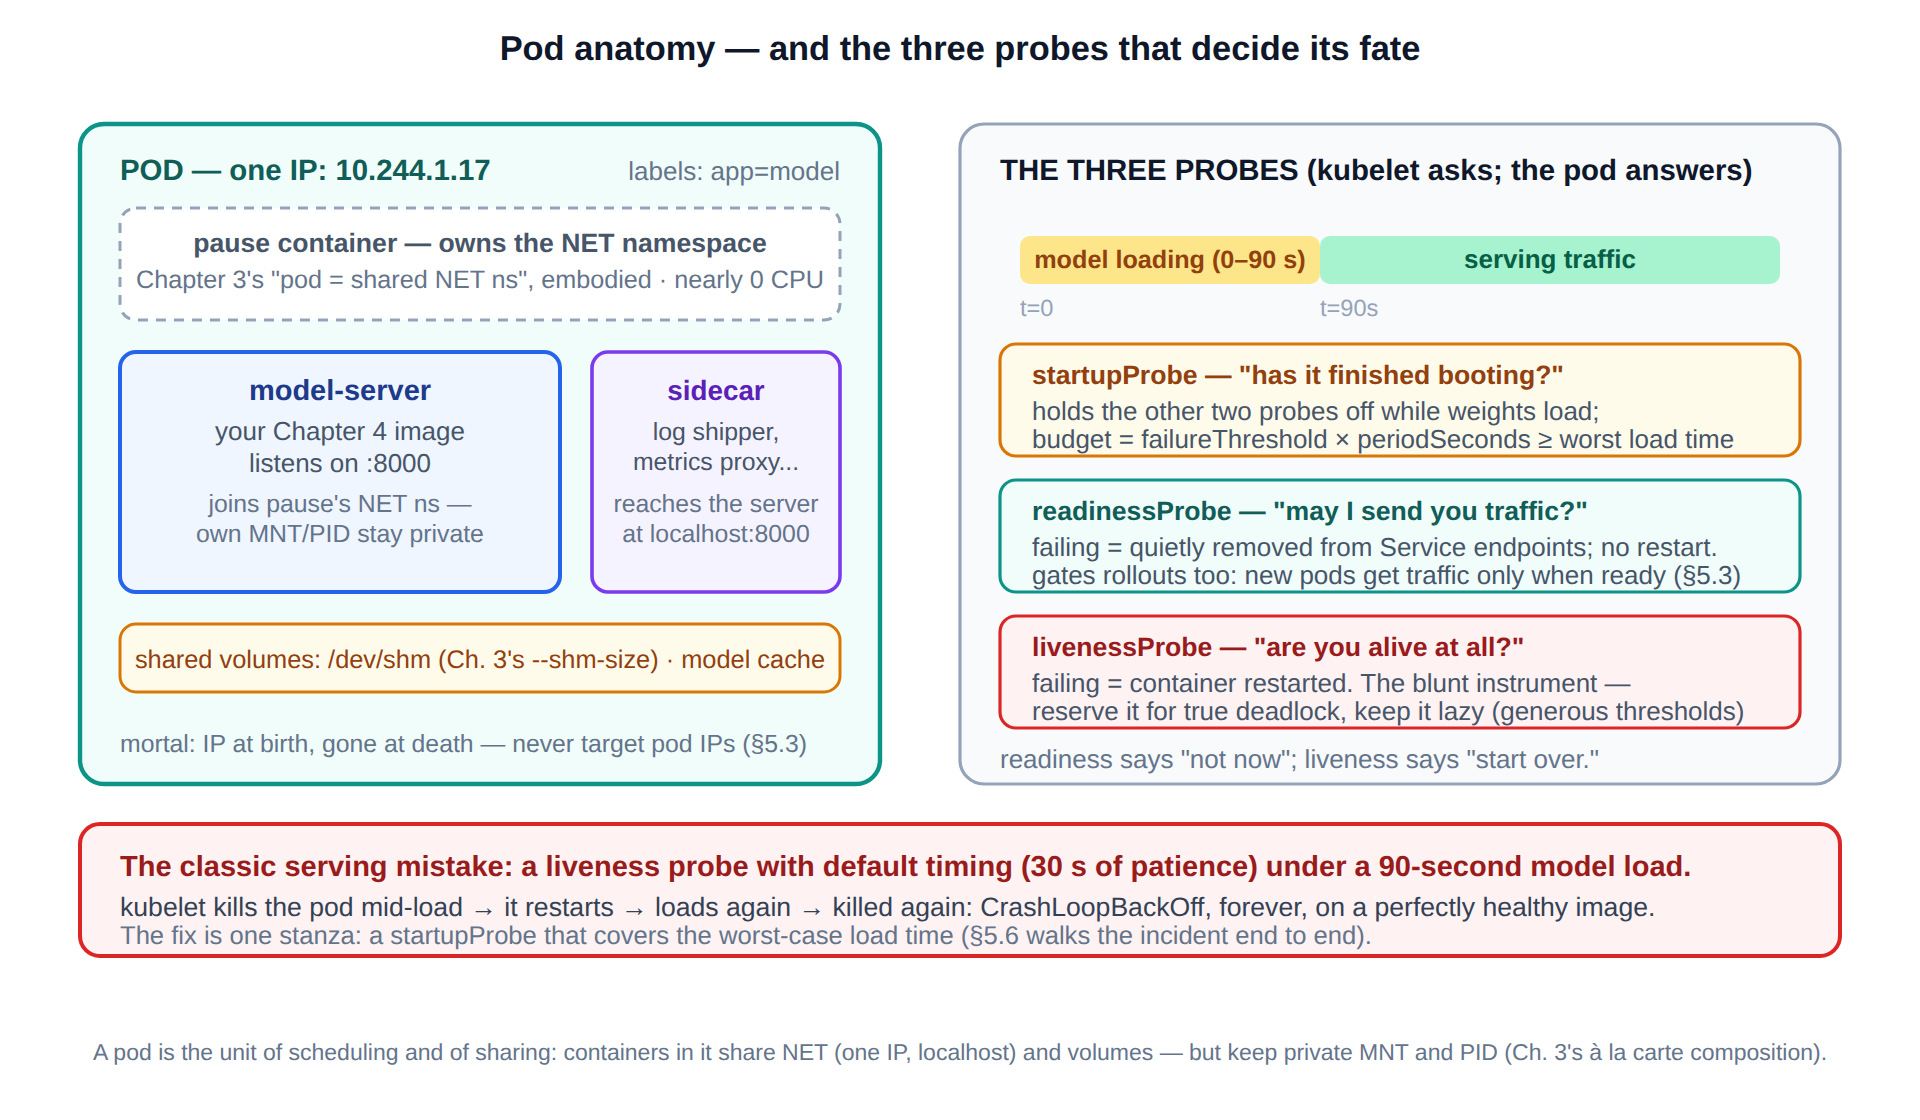
\includegraphics{figures/fig5-3_pod.png}}\\[3pt]
  \figcaption{그림 5-3  파드 구조(왼쪽): pause가 공유 네임스페이스를 소유하고 컨테이너가 합류한다. 세 가지 프로브(오른쪽): 시작 프로브는 모델 로딩을 보호하고, 준비 상태는 트래픽을 제어하며, 활성 상태는 실제로 죽은 프로세스를 재시작한다.}
\end{tbbfigure}

\subsection*{실제로 작성할 매니페스트}

강의에서 사용할 모델 서버의 전체 Deployment 매니페스트다. §5.4와 §5.6이 각각 여기의 한 구절을 바탕으로 절 하나를 전개하므로, 한 줄씩 읽어 볼 가치가 있다.

\begin{terminalbox}
\begin{Verbatim}[breaklines=true,breakanywhere=true,fontsize=\small,formatcom=\color{tbbtermfg},codes=\tbbcodeactive]
apiVersion: apps/v1
kind: Deployment
metadata:
  name: model-server
spec:
  replicas: 3
  selector:
    matchLabels: { app: model }
  template:
    metadata:
      labels: { app: model }        # must match selector - membership tag
    spec:
      terminationGracePeriodSeconds: 30   # Ch. 3's SIGTERM tape, the knob
      containers:
      - name: server
        image: registry.example.com/team/model-server:v7
        ports: [ { containerPort: 8000 } ]
        resources:                  # sec. 5.4 lives here
          requests: { cpu: "1", memory: 1.2Gi }
          limits:   { cpu: "2", memory: 1.75Gi }
        startupProbe:               # covers the model load
          httpGet: { path: /healthz, port: 8000 }
          periodSeconds: 5
          failureThreshold: 36      # 36 x 5s = 3 min of grace
        readinessProbe:             # gates traffic
          httpGet: { path: /ready, port: 8000 }
          periodSeconds: 5
        livenessProbe:              # restarts the truly dead
          httpGet: { path: /healthz, port: 8000 }
          periodSeconds: 10
          failureThreshold: 3
\end{Verbatim}
\end{terminalbox}
\figcaption{터미널 기록 5-3  강의에서 사용할 Deployment 매니페스트. 세 구절이 핵심 역할을 한다. 레이블(구성원 자격), 리소스(§5.4), 프로브(아래와 §5.6)다.}

\begin{terminalbox}
\begin{Verbatim}[breaklines=true,breakanywhere=true,fontsize=\small,formatcom=\color{tbbtermfg},codes=\tbbcodeactive]
$ kubectl apply -f model-server.yaml
deployment.apps/model-server created
$ kubectl get pods -o wide
NAME                            READY  STATUS    IP            NODE
model-server-7d4b9c6f5-8xk2p    1/1    Running   10.244.1.17   node-a
model-server-7d4b9c6f5-tq9wz    1/1    Running   10.244.2.31   node-b
model-server-7d4b9c6f5-fh5m8    0/1    Running   10.244.1.44   node-a
# 0/1 = running but not READY: the model is still loading.
# readiness is failing on purpose - and no traffic arrives yet.
\end{Verbatim}
\end{terminalbox}
\figcaption{터미널 기록 5-4  적용되어 여러 노드에 배치된 모습. 세 번째 파드에 주목하자. Running은 프로세스가 실행 중이라는 뜻이고, READY는 서빙할 준비가 되었다는 뜻이다. 둘 사이의 간격이 모델 로딩 시간이다.}

\subsection*{프로브: 세 질문과 서로 다른 세 결과}

kubelet은 모든 컨테이너에 세 가지 질문을 계속 던진다. 서빙 시스템의 생사는 이 답을 구별하는 데 달려 있다. \textbf{startupProbe}는 "부팅을 마쳤는가?"를 묻는다. 모델 때문에 시작이 느려지는 상황을 위해 존재하며, 실행되는 동안 다른 두 프로브(probe)는 중지된다. 예산(\code{failureThreshold × periodSeconds}; 터미널 기록 5-3에서는 3분)은 최악의 가중치 로딩 시간을 포괄해야 한다. \textbf{readinessProbe}는 "트래픽을 보내도 되는가?"를 묻고, 오직 Service 엔드포인트의 구성원 자격만 제어한다. 준비 상태 검사 실패는 아무것도 재시작하지 않는다. 조용히 파드를 로테이션에서 제외하며, 이는 로딩 중이거나 과부하 상태이거나 처리 중인 요청을 비우는 동안 원하는 동작이다. \textbf{livenessProbe}는 "살아 있기는 한가?"를 묻는 둔중한 도구다. 실패하면 컨테이너를 종료하고 재시작한다. 의존성이 아니라 프로세스 자체의 상태(이벤트 루프의 응답 여부)를 검사해야 하며, 충분히 긴 주기와 넉넉한 임계값을 두어 \textit{느긋하게} 동작해야 한다.

이제 대표적인 서빙 사고를 한 문장으로 설명할 수 있다. 기본 대기 시간으로 설정된 활성 상태 프로브가 모델 로딩에 90초가 걸리는 서버를 검사하면, 로딩 중인 컨테이너를 영원히 죽인다. \textbf{아무 문제가 없는 이미지에서 CrashLoopBackOff가 발생한다.} 실제 현장에서 틀림없이 만날 문제이므로 §5.6에서 터미널 기록과 함께 전체 사고를 재현한다. 예방책은 위의 startupProbe 설정이고, 진단 습관은 터미널 기록 5-4의 구분이다. Running은 Ready가 아니며, 어느 쪽도 죽었다는 뜻은 아니다.

\subsection*{Deployment: 버전이 있는 플릿과 무중단 롤아웃}

Deployment는 파드 템플릿 버전마다 하나씩 존재하는 ReplicaSet을 관리한다(템플릿 해시는 터미널 기록 5-1의 파드 이름에 그대로 나타난다). 새 이미지 태그나 새 메모리 상한처럼 템플릿의 무엇이든 바꾸면 Deployment는 \textit{새} ReplicaSet을 만들고 정해진 속도로 기존 파드와 새 파드를 교대한다. 속도는 전환 중 추가로 존재할 수 있는 수를 뜻하는 \code{maxSurge}와 비어 있어도 되는 수를 뜻하는 \code{maxUnavailable}이 결정한다. 서빙에 적합한 설정은 \code{maxSurge: 1, maxUnavailable: 0}이다. 용량을 절대 떨어뜨리지 않고, 하나를 추가해 \textbf{Ready}가 될 때까지 기다린 뒤 하나를 제거한다. 여기서 "Ready가 될 때까지 기다린다"는 문구가 핵심이다. \textbf{롤아웃의 속도는 준비 상태가 결정한다.} 새 버전이 끝내 준비 상태가 되지 않으면 추가 파드 하나에서 롤아웃이 멈춘다. 기존 버전은 계속 서빙하고 장애 영향 범위는 파드 하나로 제한된다. 시스템이 조용히 사용자의 실수로부터 사용자를 구해 주는 셈이다.

\begin{terminalbox}
\begin{Verbatim}[breaklines=true,breakanywhere=true,fontsize=\small,formatcom=\color{tbbtermfg},codes=\tbbcodeactive]
$ kubectl set image deployment/model-server server=.../model-server:v8
deployment.apps/model-server image updated
$ kubectl rollout status deployment/model-server
Waiting for rollout: 1 out of 3 new replicas are available...
$ kubectl get pods
NAME                            READY   STATUS        RESTARTS   AGE
model-server-7d4b9c6f5-8xk2p    1/1     Running       0          2d
model-server-7d4b9c6f5-tq9wz    1/1     Terminating   0          2d
model-server-6f8d5b9c44-2mwpx   1/1     Running       0          38s
model-server-6f8d5b9c44-9qk7d   0/1     Running       0          6s
# surge pod loading; an old pod drains only after a new one is Ready.
# regret it? one command points back at the old ReplicaSet:
$ kubectl rollout undo deployment/model-server
\end{Verbatim}
\end{terminalbox}
\figcaption{터미널 기록 5-5  진행 중인 롤링 업데이트. v8 파드는 Ready가 되는 대로 합류하고, 그제야 v7 파드가 종료된다. 롤백은 규모 0으로 유지해 둔 이전 ReplicaSet을 다시 가리키는 일이다.}

제3장의 관점으로 \code{Terminating} 파드를 보자. kubelet은 \textbf{PID 1에 SIGTERM}을 보내고 \code{terminationGracePeriodSeconds}만큼 기다린 뒤(매니페스트에서는 30으로 설정했다) SIGKILL을 보낸다. exec 형식 CMD, 새 요청 수락을 멈추고 처리 중인 요청을 비우는 핸들러, 필요하다면 tini까지 §3.2에서 배운 모든 것이 \code{Terminating} 시간을 클라이언트에게 보이지 않게 한다. Kubernetes가 우아한 종료(graceful shutdown)를 해결한 것은 아니다. 단지 종료를 \textit{스케줄링}한다. 이 강의의 나머지 기간 동안 모든 롤아웃, 노드 비우기, 축소 때마다 실제 작업은 여전히 핸들러가 수행한다.

\subsection*{Service: 사라질 파드 앞에 놓는 안정적인 이름 하나}

파드는 가축과 같다. 태어날 때 IP를 받고 죽을 때 잃는다. 터미널 기록 5-5에서 죽음이 얼마나 일상적인지 보았다. 클라이언트에게 이를 일일이 따라가라고 할 수는 없다. 해결책은 \textbf{Service}다. 현재 \textbf{레이블 셀렉터(selector)}와 일치하면서 준비 상태 검사를 통과한 파드 앞에 안정적인 가상 IP와 DNS 이름(\code{model-svc.ml.svc.cluster.local}, CoreDNS가 제공)을 둔다. 일치하는 파드의 IP가 \textbf{엔드포인트} 목록을 구성하고 컨트롤러가 이를 실시간으로 갱신한다. \textbf{kube-proxy}는 가상 IP로 들어온 연결을 정상 백엔드 하나로 DNAT 변환하도록 노드의 패킷 경로(iptables 또는 IPVS)를 프로그래밍한다. 제3장의 \code{-p 8080:8000} 패킷 경로에서 정확히 같은 메커니즘을 만났다. 공개 포트는 NAT 규칙 하나였고, Service는 같은 기법을 클러스터 전체에 건강 상태를 반영해 적용한다(그림 5-4). MSA 관점에서는 \textbf{플랫폼이 해결한 서비스 디스커버리}다. 소비자는 이름만 알 뿐 토폴로지는 알 필요가 없다.

\begin{tbbfigure}
  \adjustbox{max width=0.94\linewidth,max totalheight=0.46\textheight}{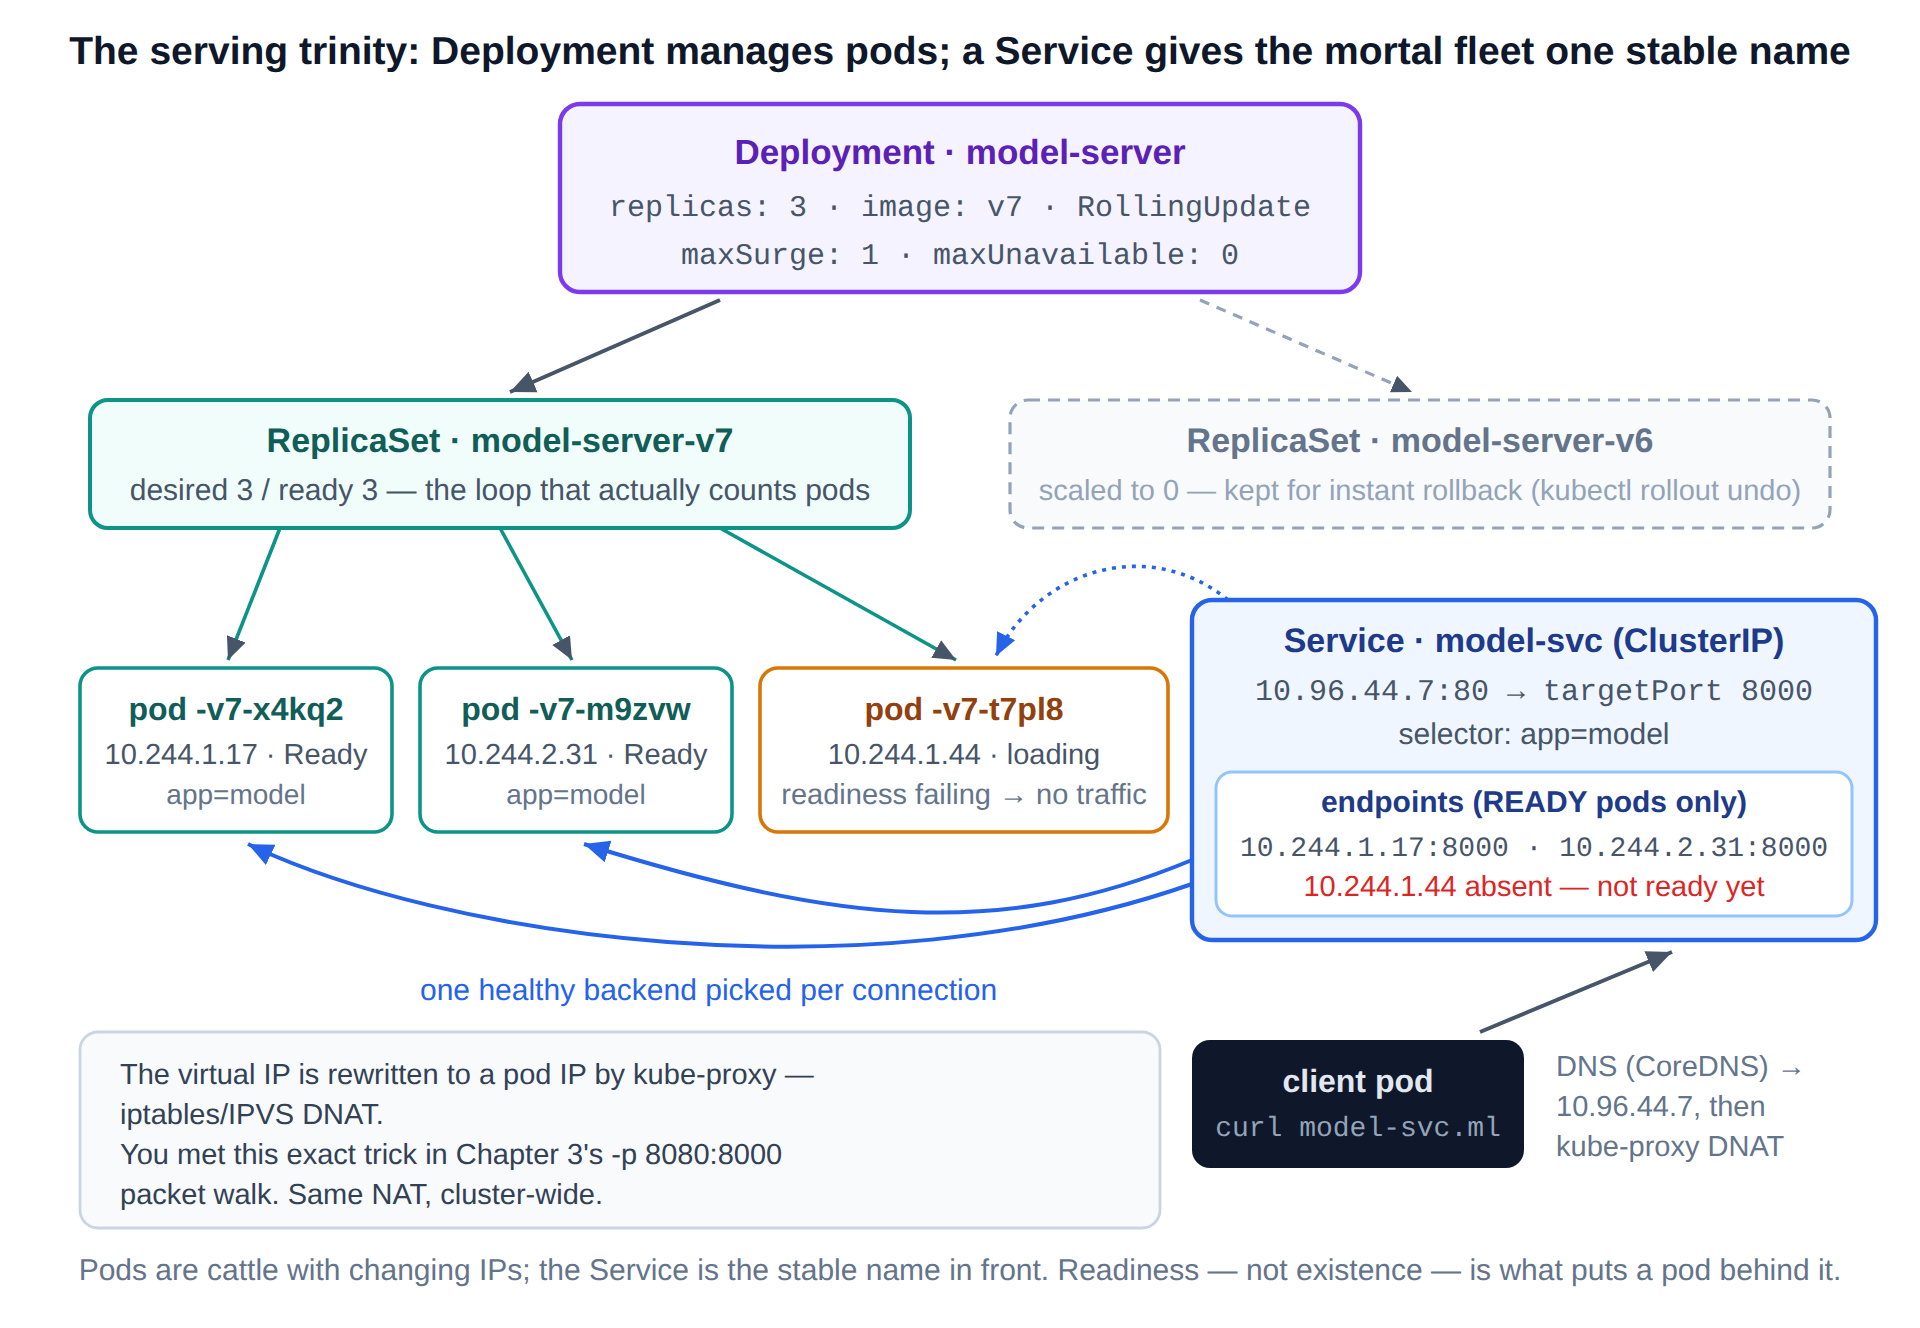
\includegraphics{figures/fig5-4_deploy_svc.png}}\\[3pt]
  \figcaption{그림 5-4  Deployment → ReplicaSet → 파드 앞에 Service가 놓인 구조. 엔드포인트 목록에는 READY 파드만 들어간다. 그래서 로딩 중인 파드와 처리 중인 요청을 비우는 파드가 트래픽에서 자동으로 빠진다.}
\end{tbbfigure}

\begin{terminalbox}
\begin{Verbatim}[breaklines=true,breakanywhere=true,fontsize=\small,formatcom=\color{tbbtermfg},codes=\tbbcodeactive]
$ kubectl expose deployment model-server --name=model-svc \
    --port 80 --target-port 8000
service/model-svc exposed
$ kubectl get svc model-svc
NAME        TYPE        CLUSTER-IP     EXTERNAL-IP   PORT(S)   AGE
model-svc   ClusterIP   10.96.44.7     <none>        80/TCP    5s
$ kubectl get endpoints model-svc
NAME        ENDPOINTS                             AGE
model-svc   10.244.1.17:8000,10.244.2.31:8000     5s
# two backends - the third pod is still loading (not Ready).
# from any pod in the cluster:
$ curl -s http://model-svc.default/predict -d '{"x": [1,2]}'
{"y": 0.87, "model": "v7"}
\end{Verbatim}
\end{terminalbox}
\figcaption{터미널 기록 5-6  플릿 앞에 놓인 Service. 가상 IP, DNS 이름, 준비 상태 프로브에 응답하는 파드만 담는 엔드포인트 목록을 제공한다.}

세 가지 Service 유형은 노출 범위를 단계적으로 넓힌다. \textbf{ClusterIP}(위 예시의 기본값)는 클러스터 내부에서만 접근할 수 있어 다른 서비스 뒤에 놓인 모델 서버에 적합하다. \textbf{NodePort}는 모든 노드에서 높은 번호의 포트(30000–32767)를 연다. minikube 실습에서 외부로 나가는 방법이다. \textbf{LoadBalancer}는 해당 노드 포트에 연결된 실제 외부 로드 밸런서를 클라우드에 요청한다. 관리형 클러스터에서 쓰는 방식이며, 6주 차에는 앞단에 API 게이트웨이, TLS, 인증을 추가한다. 지금 기억할 점이 하나 있다. Service는 요청이 아니라 \textit{연결}을 로드 밸런싱한다. 스트리밍이나 gRPC 멀티플렉싱처럼 오래 유지되는 연결은 이를 무력화할 수 있으며, 이 문제는 11주 차 LLM 스트리밍에서 다시 등장한다.

세 축이 아직 기억에 생생할 때 습관을 하나 더 들이자. 바로 \textbf{네임스페이스}다. 이름, 할당량, 접근 권한의 범위를 나눈다. 실습에서는 모든 것을 \code{default}가 아니라 \code{ml}이라는 네임스페이스 안에 만든다. 실제로 접할 모든 클러스터가 이런 식으로 나뉘며, 13주 차의 CI/CD 파이프라인도 환경별 네임스페이스에 배포하기 때문이다.

\begin{calloutbox}{tbbpurple}{tbbpurplefill}
{\normalsize\bfseries\color{tbbpurple}생각해 보기}\par\vspace{3pt}
\begin{tbbitemize}
  \item model-server-v7과 실험용 v8이라는 두 Deployment에 실수로 모두 app=model 레이블이 붙었고, 하나의 Service가 app=model을 선택한다. 클라이언트가 정확히 무엇을 경험하는지, 어떤 구성 요소도 오류를 알리지 않는 이유는 무엇인지, 어디에서 이 상황을 가장 먼저 확인할 수 있는지 설명하자. (이 구성을 의도적으로 만들면 카나리라 부른다. 13주 차에서 다룬다.)
  \item 롤링 업데이트는 컨테이너가 시작되기만을 기다리는 것이 아니라 준비 상태를 기다린다. 전체 트래픽을 받는 상황에서 로딩에 90초가 걸리는 모델에 maxSurge: 1, maxUnavailable: 0을 적용하되 컨테이너 시작 여부만 기준으로 삼으면 어떤 구체적인 재난이 생기는지 구성해 보자.
  \item 파드는 살아 있고(활성 상태 검사 통과) 준비는 끝내 되지 않으며(준비 상태 검사 실패) 재시작도 되지 않은 채 무기한 머물 수 있다. 이 끝나지 않는 상태가 기능인 이유를 논증한 뒤, 의도하지 않았을 때 §5.6의 어떤 실패가 되는지 말해 보자.
\end{tbbitemize}
\end{calloutbox}

\section{requests, limits, QoS: 플릿 규모로 확장한 제3장}

터미널 기록 5-3의 \code{resources:} 구절은 여덟 줄에 불과하지만, 나머지 매니페스트 전체를 합친 것보다 운영상 중요하다. 이해하기 까다로운 핵심은 \textbf{서로 다른 두 가지 일을 하는 두 시스템이 이 구절을 읽는다}는 점이다(그림 5-5). 배치 시점에 \textit{스케줄러}는 \textbf{requests}를 산술 값으로 읽는다. 노드의 \textbf{allocatable} 용량에서 이미 배치된 requests의 합을 빼고도 새 파드의 requests를 감당할 수 있으면 파드가 들어간다. requests는 그저 계획을 위한 숫자다. \textbf{런타임에는 절대 강제되지 않는다.} 노드에 여유가 있으면 1 CPU를 요청한 파드가 3을 사용해도 된다. 반면 \textit{kubelet}이 읽는 \textbf{limits}는 제4장의 런타임 스택을 거쳐 제3장의 cgroup 파일로 정확히 변환되며, 커널이 매 밀리초마다 강제한다.

\begin{tbbfigure}
  \adjustbox{max width=0.94\linewidth,max totalheight=0.46\textheight}{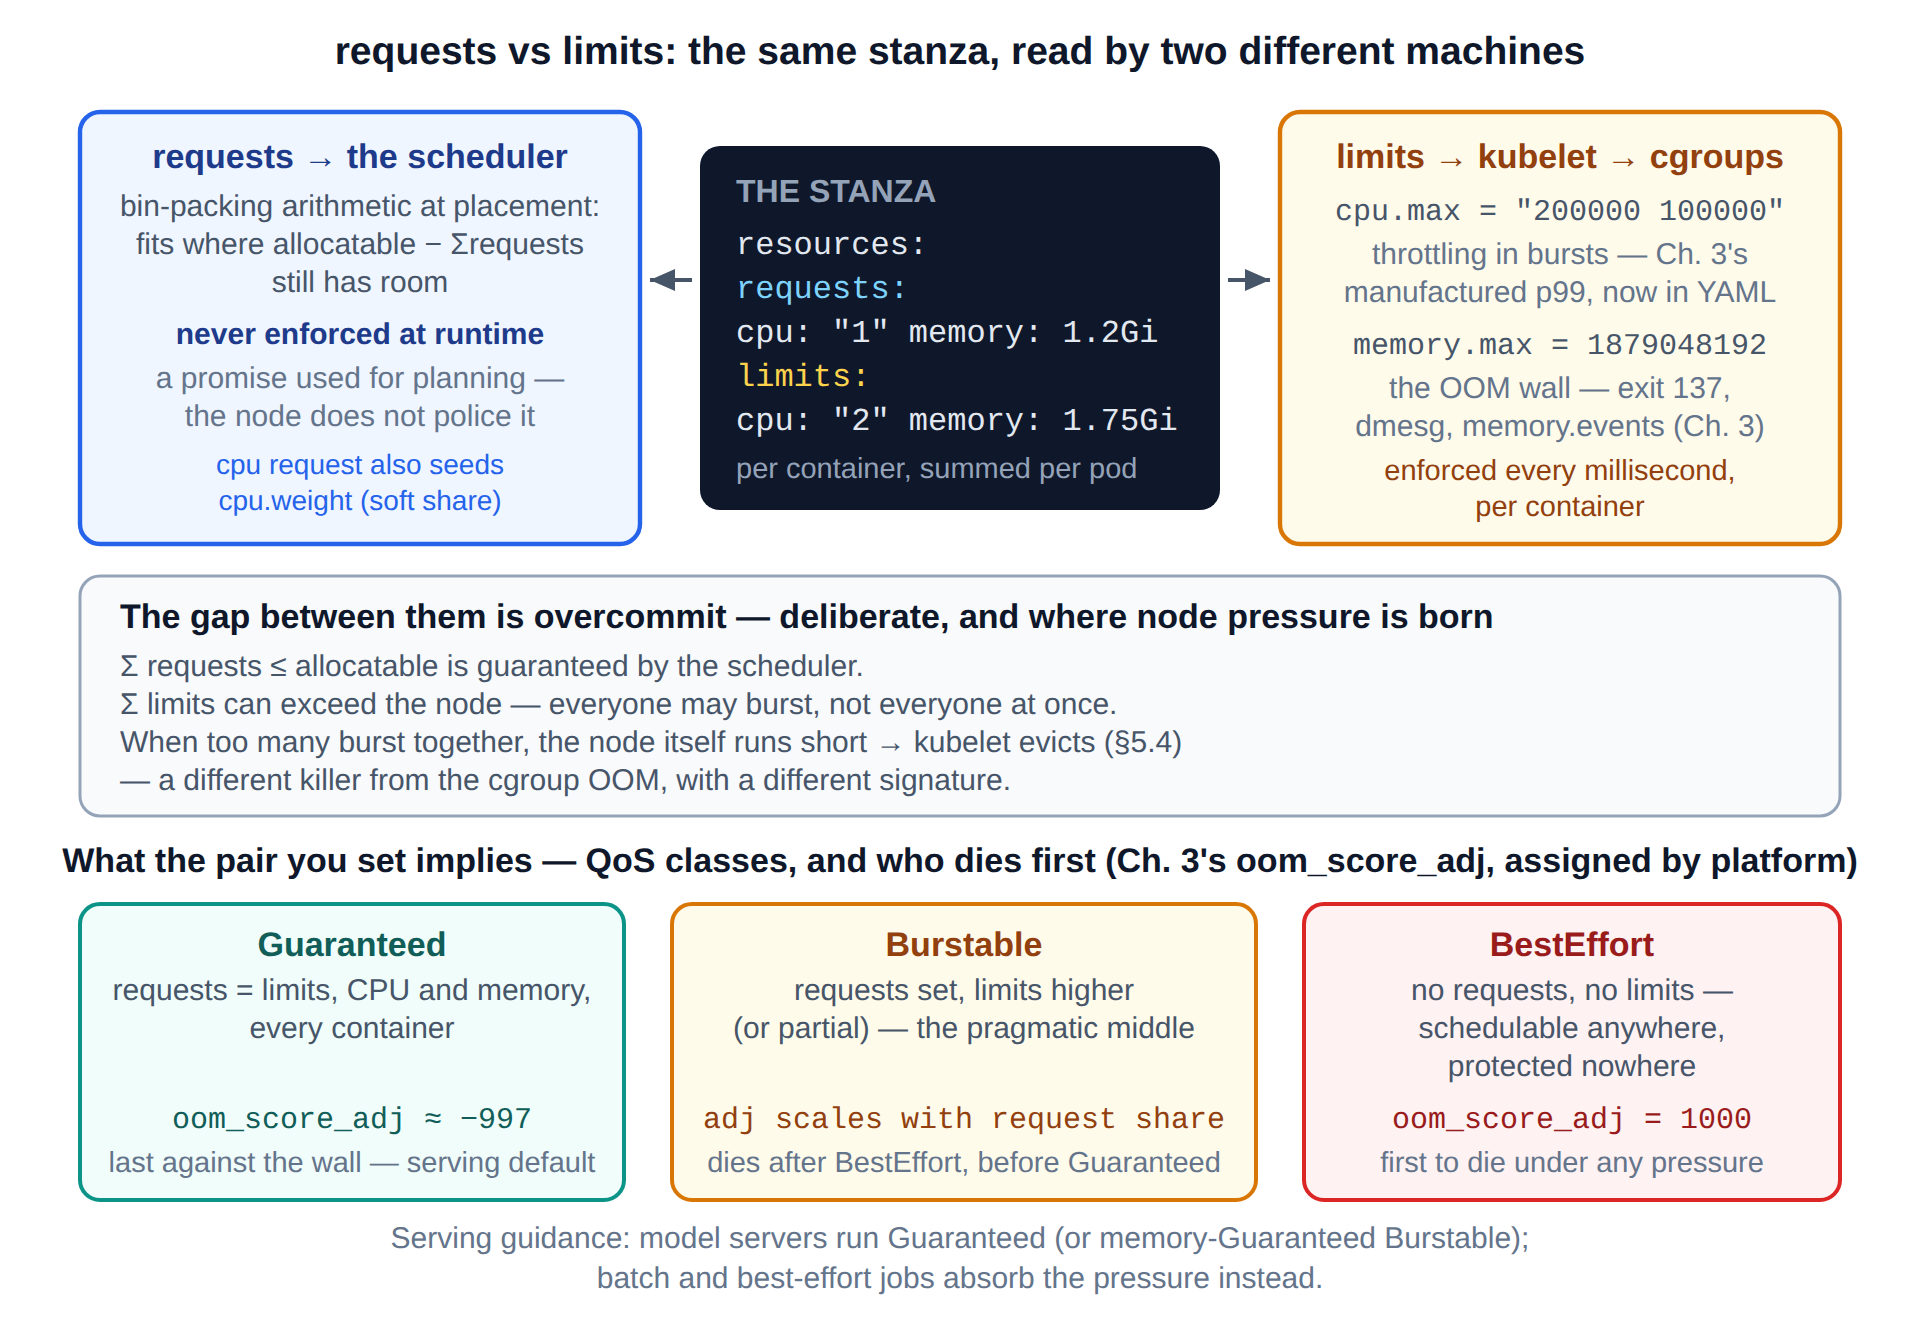
\includegraphics{figures/fig5-5_requests_limits.png}}\\[3pt]
  \figcaption{그림 5-5  하나의 구절을 읽는 두 주체. requests는 스케줄러의 빈 패킹에 쓰이고, limits는 cpu.max와 memory.max가 된다. 둘 사이의 간격은 의도적인 오버커밋이며, 노드 압박이 시작되는 지점이기도 하다.}
\end{tbbfigure}

\subsection*{핵심을 증명하는 기록: YAML을 넣으면 cgroup 파일이 나온다}

제3장은 호스트에서 Docker 컨테이너를 조사해 cgroup 파일이 연결된 프로세스를 찾아내며 시작했다. Kubernetes에서 같은 조사를 수행하면 이 장의 핵심 주장이 완성된다.

\begin{terminalbox}
\begin{Verbatim}[breaklines=true,breakanywhere=true,fontsize=\small,formatcom=\color{tbbtermfg},codes=\tbbcodeactive]
$ kubectl get pod model-server-7d4b9c6f5-8xk2p \
    -o jsonpath='{.spec.nodeName} {.status.qosClass}'
node-a Burstable
$ minikube ssh                        # onto the node itself
node-a $ ps aux | grep uvicorn        # the server is just a process (Ch. 3)
root  41320  2.1  7.8  ...  uvicorn serve:app --port 8000
node-a $ cat /proc/41320/cgroup
0::/kubepods.slice/kubepods-burstable.slice/kubepods-...-pod9f31.slice/...
node-a $ cd /sys/fs/cgroup/kubepods.slice/kubepods-burstable.slice/...
node-a $ cat memory.max
1879048192                            # = 1.75Gi, your YAML, in bytes
node-a $ cat cpu.max
200000 100000                         # = limits.cpu "2", Ch. 3 grammar
node-a $ cat cpu.weight
39                                    # from requests.cpu "1" - soft share
\end{Verbatim}
\end{terminalbox}
\figcaption{터미널 기록 5-7  연결 고리를 직접 완성했다. YAML의 limits는 노드의 memory.max와 cpu.max가 되었고, CPU 요청량은 cpu.weight가 되었다. Kubernetes는 제3장의 앞에 데이터베이스를 붙인 시스템이다.}

세 파일을 제3장과 연결해 읽으면 모든 동작이 자연스럽게 따라 나온다. \code{memory.max = 1879048192}는 파드가 \textbf{같은 OOM 킬러, 같은 exit 137, 같은 dmesg의 자백, 같은 크기 산정법}을 만난다는 뜻이다. §3.6이 그대로 적용되고 \code{kubectl describe}에는 \code{Last State: OOMKilled}로 나타난다. \code{cpu.max = "200000 100000"}는 파드가 \textbf{버스트 중에 스로틀링될 수 있음}을 뜻한다. §3.3에서 인위적으로 만든 p99가 이제 YAML 한 줄로 설정된다. requests에서 파생된 \code{cpu.weight}는 경합이 있을 때만 영향을 주는, 정중하고 작업 보존적인 지분이다. 기억해야 할 표는 다음과 같다.

\begin{tbbtablewrap}
  \begin{tabular}{@{}>{\raggedright\arraybackslash}m{\dimexpr 0.3085\tbltextwidth-2\tabcolsep\relax} >{\raggedright\arraybackslash}m{\dimexpr 0.3511\tbltextwidth-2\tabcolsep\relax} >{\raggedright\arraybackslash}m{\dimexpr 0.3404\tbltextwidth-2\tabcolsep\relax}@{}}
  \arrayrulecolor{tbbnavy}\specialrule{1pt}{0pt}{0pt}
  \rowcolor{tbbtablehead}{\centering \bfseries\color{tbbnavy}작성 내용(YAML)} & {\centering \bfseries\color{tbbnavy}변환 결과} & {\centering \bfseries\color{tbbnavy}성격} \\
  \arrayrulecolor{tbbnavy}\specialrule{0.7pt}{0pt}{2pt}
  {requests.cpu: "1"} & {스케줄러 산술 + cpu.weight} & {계획 + 유연한 지분, 작업 보존적} \\
  \arrayrulecolor{tbbtableborder}\hline
  {requests.memory: 1.2Gi} & {스케줄러 산술(+ 퇴거 순위)} & {계획에만 사용, 커널 객체 없음} \\
  \arrayrulecolor{tbbtableborder}\hline
  {limits.cpu: "2"} & {\textcolor{tbbamberdark}{cpu.max = "200000 100000"}} & {엄격한 할당량, 버스트에서 스로틀링(§3.3)} \\
  \arrayrulecolor{tbbtableborder}\hline
  {limits.memory: 1.75Gi} & {\textcolor{tbbred}{memory.max = 1879048192}} & {엄격한 벽, OOM killer(§3.6)} \\
  \arrayrulecolor{tbbtableborder}\hline
  {nvidia.com/gpu: 1} & {디바이스 플러그인 할당(§5.5)} & {정수, cgroup이 없어 중재할 커널 기능 없음} \\
  \arrayrulecolor{tbbnavy}\specialrule{1pt}{2pt}{0pt}
  \end{tabular}\par
  \figcaption{표 5-1  한 줄씩 살펴보는 변환 관계}
\end{tbbtablewrap}

\subsection*{CPU: request는 넉넉하게, limit는 신중하게}

CPU에서 두 설정값은 제3장에서 본 서로 다른 두 성격을 이어받으며, 서빙 지침도 기계적으로 도출된다. request는 \textit{예약}이다. 배치 위치를 결정하고, \code{cpu.weight}를 통해 경합 중에는 비례 배분의 하한을 보장하면서도 이웃이 놀 때는 자원을 낭비하지 않는다. limit는 \code{cpu.max}라는 \textit{상한}이다. §3.3의 계산에서 상한이 꼬리 지연 시간에 미치는 영향을 보았다. CPU 시간 30 ms가 필요한 요청은 0.2-CPU 할당량 아래에서 110–190 ms가 걸리지만 프로파일러에는 원인이 보이지 않는다. 따라서 \textbf{CPU requests는 정직하게 설정}해야 한다. 이웃 워크로드 간섭이 있을 때 p99를 지키는 보험이기 때문이다. 반면 지연 시간에 민감한 파드에서는 \textbf{CPU limits를 신중하게 사용}해야 한다. 버스트를 흡수하는 데 쓰인 유휴 코어가 p99 구간에서 스로틀링되는 것보다 저렴하다. 다만 현실에는 두 가지 복잡한 점이 있다. 플랫폼 팀이 비용 관리와 폭주 방지를 위해 limits를 \textit{요구}할 때가 많고, 다음 문단에서 볼 Guaranteed QoS는 requests = limits를 요구한다. 일정한 성능과 QoS가 모두 필요한 팀은 두 값을 똑같이 넉넉하게 잡거나 kubelet의 정적 CPU 매니저 정책을 사용한다. 이 정책은 Guaranteed 등급의 정수-CPU 파드에 \textit{전용 코어}를 준다. 제2장의 전용 코어 개념이 kubelet에서 다시 등장한 것이다.

\subsection*{메모리: 간격, 압박, 두 번째 처형자}

메모리에서는 requests와 limits의 간격을 설명하는 별도 어휘가 필요하다. 스케줄러는 노드마다 Σrequests ≤ allocatable을 보장하지만 limits에는 관여하지 않으므로 \textbf{Σlimits가 노드 용량을 넘는 일은 흔하다.} 이것이 오버커밋이며 기능이다. 모두가 동시에 버스트하지는 않으리라는 가정 아래 누구나 버스트할 수 있게 한다. 이 가정이 틀리면, 예를 들어 여러 레플리카의 사용량이 함께 치솟으면(§3.6에서 보았듯 추론 메모리는 \textit{본질적으로 급격히 변한다}) 개별 파드가 자기 벽에 닿기 전에 \textbf{노드 자체}의 메모리가 부족해진다. 커널의 노드 수준 OOM 킬러에 맡기면 혼란스러우므로 Kubernetes는 질서를 택한다. \textbf{kubelet이 퇴거}를 수행한다. QoS 클래스와 requests 초과 사용량을 기준으로 희생 대상을 고르고 정상적으로 종료한 뒤 \code{Evicted}로 표시한다. 이제 서로 다른 두 처형자를 알게 되었다. 둘을 구별하는 능력은 §5.6의 핵심이다.

\begin{tbbtablewrap}
  \begin{tabular}{@{}>{\raggedright\arraybackslash}m{\dimexpr 0.2340\tbltextwidth-2\tabcolsep\relax} >{\raggedright\arraybackslash}m{\dimexpr 0.3830\tbltextwidth-2\tabcolsep\relax} >{\raggedright\arraybackslash}m{\dimexpr 0.3830\tbltextwidth-2\tabcolsep\relax}@{}}
  \arrayrulecolor{tbbnavy}\specialrule{1pt}{0pt}{0pt}
  \rowcolor{tbbtablehead}{\centering \bfseries\color{tbbnavy}} & {\centering \bfseries\color{tbbnavy}cgroup OOM 종료(제3장)} & {\centering \bfseries\color{tbbnavy}노드 압박(node pressure) 퇴거} \\
  \arrayrulecolor{tbbnavy}\specialrule{0.7pt}{0pt}{2pt}
  {\textbf{발동 조건}} & {파드가 자기 memory.max를 초과} & {노드 메모리 부족(오버커밋 가정 실패)} \\
  \arrayrulecolor{tbbtableborder}\hline
  {\textbf{처형자}} & {커널 OOM 킬러 — SIGKILL} & {kubelet — 파드를 정상 절차로 종료} \\
  \arrayrulecolor{tbbtableborder}\hline
  {\textbf{영향 범위}} & {컨테이너 하나} & {QoS 순서에 따라 고른 희생 대상, 노드 전체} \\
  \arrayrulecolor{tbbtableborder}\hline
  {\textbf{징후}} & {\textcolor{tbbred}{OOMKilled · exit 137 · dmesg}} & {\textcolor{tbbpurple}{상태 Evicted · "노드 메모리가 부족함"}} \\
  \arrayrulecolor{tbbtableborder}\hline
  {\textbf{우선 해결책}} & {최댓값에 맞춰 크기 조정 또는 배치 제한(§3.6)} & {정직한 requests, 서빙에 Guaranteed QoS 적용} \\
  \arrayrulecolor{tbbnavy}\specialrule{1pt}{2pt}{0pt}
  \end{tabular}\par
  \figcaption{표 5-2  두 처형자와 두 가지 징후}
\end{tbbtablewrap}

\subsection*{QoS 클래스: 누가 먼저 죽을지도 설정이다}

kubelet의 퇴거 순서와, 그 단계까지 간다면 노드 OOM 킬러의 점수는 추측으로 정해지지 않는다. 플랫폼이 requests/limits 패턴에 따라 할당하는 제3장의 \code{oom\_score\_adj}다. 모든 컨테이너의 CPU와 메모리에서 requests = limits인 \textbf{Guaranteed}는 ≈ −997을 받아 거의 건드릴 수 없다. 아무것도 설정하지 않은 \textbf{BestEffort}는 +1000을 받아 언제나 가장 먼저 희생된다. 그 사이에 있는 \textbf{Burstable}은 사용량이 requests를 얼마나 초과했는지에 따라 점수가 달라진다. 서빙에 적용할 원칙은 명확하다. \textbf{모델 서버는 Guaranteed로 실행}해야 한다. 최소한 memory requests = limits로 맞춘다. 그러면 오버커밋된 노드가 압박을 받을 때 p99를 책임지는 파드가 아니라 배치 작업과 BestEffort 실험이 죽는다. (Kubernetes에는 이와 독립적인 두 번째 설정인 PriorityClass도 있다. 이는 \textit{워크로드 사이의 선점과 퇴거} 순서를 정하고, QoS는 \textit{한 노드에서 종료할 우선순위}를 정한다. 12주 차 오토스케일링에서는 둘 다 사용한다.)

\begin{calloutbox}{tbbblue}{tbbbluefill}
{\normalsize\bfseries\color{tbbblue}계산 예제 — 직접 해 보는 노드 패킹}\par\vspace{3pt}
범용 8-vCPU / 32 GiB 노드를 생각해 보자. 시스템과 kubelet 예약분을 빼면 \textbf{allocatable(할당 가능 용량)은 ≈ 7.5 vCPU 및 29 GiB}다(터미널 기록 5-8에서 확인 위치를 보여 준다). 노드마다 실행되는 데몬(로그 수집기, 모니터링 에이전트, kube-proxy)은 ≈ 0.3 vCPU 및 0.5 GiB를 요청한다. 강의 모델 서버의 requests는 \code{cpu: 1, memory: 1.2Gi}이고 limits는 2 / 1.75Gi다.

\begin{tbbitemize}
  \item \textbf{CPU 계산:} (7.5 − 0.3) / 1 = CPU requests 기준으로 \textbf{레플리카 7개}가 들어간다.
  \item \textbf{메모리 계산:} (29 − 0.5) / 1.2 ≈ 메모리 requests 기준으로 \textbf{레플리카 23개}가 들어간다.
\end{tbbitemize}

이 워크로드에서 노드는 \textbf{CPU 병목}이다. 노드마다 레플리카 7개가 들어가고 메모리는 남는다. 따라서 메모리가 많은 인스턴스 유형에 비용을 더 내면 낭비다. 제1장의 비용 관점처럼 인스턴스는 제약이 되는 차원에 맞춰 골라야 한다. 이제 오버커밋 노출을 확인하자. 레플리카 7개 × limits = 14 vCPU 및 12.25 GiB다. CPU limits(14)는 allocatable(7.5)을 넘지만 합법이다. 동시에 버스트하면 requests에 비례해 cpu.weight가 분배하며, p99는 requests가 얼마나 정직한지에 달렸다. 메모리 limits(12.25 GiB)는 29 GiB보다 훨씬 작다. 이 패킹은 원리상 노드 메모리 압박을 일으킬 수조차 없으며, 서빙 노드에 의도적으로 적용한 보수적인 자세다.

\code{cpu: 2, memory: 9Gi}를 요청하는 7B 매개변수 INT8 LLM 서버에 같은 계산을 적용해 보자. 이제 메모리가 제약이 되어 (29 − 0.5) / 9 = \textbf{레플리카 3개}가 들어가고, 적합한 노드 계열은 컴퓨팅 최적화에서 메모리 최적화로 바뀐다. 2분간 나눗셈만 해도 인스턴스 계열을 결정할 수 있다. 12주 차 FinOps 절은 바로 이 습관을 바탕으로 전체 비용 모델을 세운다.
\end{calloutbox}

\vspace{3.0pt}

\begin{calloutbox}{tbbpurple}{tbbpurplefill}
{\normalsize\bfseries\color{tbbpurple}생각해 보기}\par\vspace{3pt}
\begin{tbbitemize}
  \item 파드가 requests(1 CPU / 1 Gi)는 설정했지만 limits는 설정하지 않았다. 이 파드의 QoS 클래스는 무엇인가? 다른 파드가 놀고 있는 노드에서 이 파드가 메모리를 누수하면 어떻게 되는가? 반대로 \textit{이웃}이 누수하면 누가 먼저 위험해지는가?
  \item 스케줄러가 limits를 완전히 무시하는 이유는 무엇인가? 오버커밋이 기능이라는 관점에서 논리를 구성한 뒤, limits를 기준으로 스케줄링하는 편이 분명히 나은 워크로드 조합 하나를 들어 보자.
  \item 계산 예제의 레플리카 7개 모두 피크 트래픽에서 nr\_throttled가 증가한다(limits.cpu 2 × 7 = 할당 가능 용량 7.5에서 14). §3.3과 이 절을 바탕으로 p99 징후를 설명하고, 비용이 서로 다른 해결책 두 가지를 제안하자.
\end{tbbitemize}
\end{calloutbox}

\section{GPU와 스케줄러}

지금까지는 노드를 서로 바꿔 쓸 수 있다고 가정했다. GPU가 등장하는 순간 배치는 비용이 큰 결정으로 바뀐다. GPU 플릿을 잘 배치했을 때와 잘못 배치했을 때의 차이는 매달 수천 달러에 이른다. CPU와 달리 \textbf{GPU에는 오버커밋이 없으므로} 실수를 오버커밋으로 흡수할 수도 없다. 이 절에서는 가장 까다로운 사례인 GPU를 중심으로 스케줄러를 살펴본다.

\subsection*{필터링, 점수화, 바인딩 — 배치 과정 자체}

스케줄러는 바인딩되지 않은 파드마다 두 단계의 과정을 수행한다(그림 5-6). \textbf{필터링}은 파드를 실행할 수 \textit{없는} 모든 노드를 제거한다. requests를 감당할 할당 가능 리소스가 부족하거나, 필요한 확장 리소스가 없거나, nodeSelector 또는 어피니티(affinity)가 맞지 않거나, 테인트를 톨러레이션하지 않는 노드가 탈락한다. 남은 노드가 실행 가능 집합이다. 이 집합이 비면 파드는 \textbf{Pending}에 머문다. 특히 \textit{이벤트 메시지는 어떤 필터에서 몇 개 노드가 실패했는지 정확히 열거한다}는 점이 중요하다(§5.6에서 실제 메시지를 읽는다). 이어서 \textbf{점수화}는 가용 영역(availability zone) 분산, 부하가 더 적거나 더 많은 노드 선호, 이미지 존재 여부 같은 유연한 선호 조건으로 실행 가능 집합의 순위를 매긴다. 마지막으로 \textbf{바인딩}이 승자의 이름을 파드 객체에 기록한다. 스케줄러의 출력은 객체 하나의 필드 하나이며, 이후 과정은 모두 §5.2의 연결 고리다.

\begin{tbbfigure}
  \adjustbox{max width=0.94\linewidth,max totalheight=0.46\textheight}{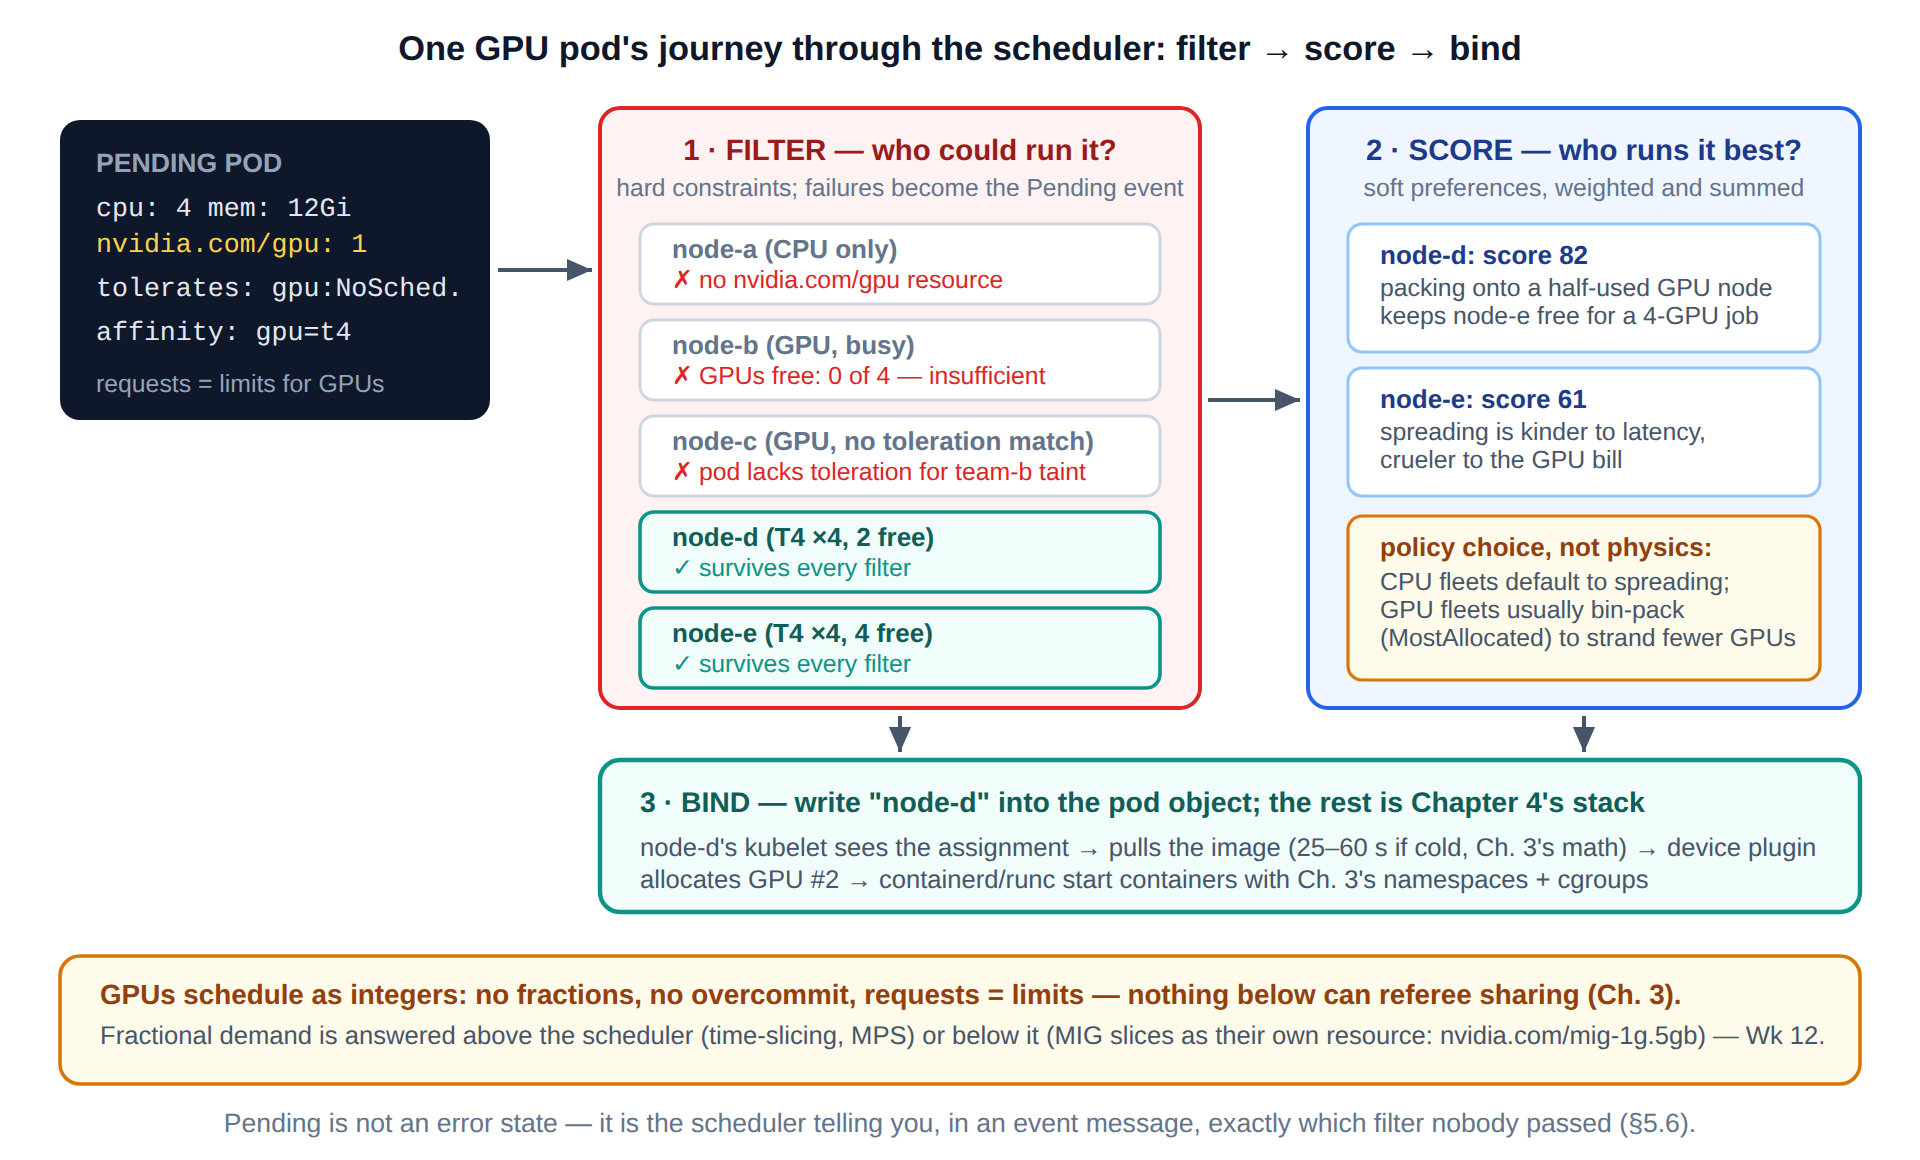
\includegraphics{figures/fig5-6_scheduler.png}}\\[3pt]
  \figcaption{그림 5-6  GPU 파드의 스케줄링 과정. 필터가 노드를 제거하고 실패 이유는 Pending 이벤트가 된다. 점수가 순위를 매기고 바인딩이 이름을 기록한다. 패킹과 분산 중 무엇을 택할지는 GPU만큼 값비싼 정책 결정이다.}
\end{tbbfigure}

\subsection*{GPU는 확장 리소스다: 정수, 오버커밋 없음, requests = limits}

GPU는 \textbf{확장 리소스}로 Kubernetes에 들어온다. 각 GPU 노드에서 실행되는 제4장의 디바이스 플러그인이 kubelet에 \code{nvidia.com/\allowbreak gpu: 4}를 알리고, kubelet이 이를 노드 용량에 보고한다. 파드는 구절 하나로 GPU를 소비한다. 이때 CPU나 메모리보다 엄격한 세 규칙이 적용된다. 수량은 \textbf{정수}여야 하고, \textbf{requests와 limits가 같아야 하며}, \textbf{어떤 경우에도 오버커밋은 없다.} 파드가 시작되면 디바이스 플러그인이 인덱스/UUID로 \textit{특정} GPU를 할당해 컨테이너에 주입한다. 제4장에서 본 \code{/\allowbreak dev/\allowbreak nvidia*} 배관이다.

\begin{terminalbox}
\begin{Verbatim}[breaklines=true,breakanywhere=true,fontsize=\small,formatcom=\color{tbbtermfg},codes=\tbbcodeactive]
# in the pod spec - the entire GPU ask:
        resources:
          limits:
            nvidia.com/gpu: 1        # integer; requests implied equal

$ kubectl describe node gpu-node-3 | sed -n '/Capacity/,/pods/p'
Capacity:
  cpu:                48
  memory:             196Gi
  nvidia.com/gpu:     4
Allocatable:
  cpu:                47
  memory:             186Gi
  nvidia.com/gpu:     4
$ kubectl describe node gpu-node-3 | grep -A4 "Allocated resources"
Allocated resources:
  Resource           Requests      Limits
  cpu                18 (38%)      36 (76%)
  memory             88Gi (47%)    120Gi (64%)
  nvidia.com/gpu     2             2          # 2 of 4 in use
\end{Verbatim}
\end{terminalbox}
\figcaption{터미널 기록 5-8  스케줄러가 보는 GPU 노드. 디바이스 플러그인이 Capacity/Allocatable에 알린 값과 현재 GPU 점유 상태가 보인다. CPU limits는 오버커밋되어 있지만 GPU는 그렇지 않다.}

왜 이렇게 엄격할까? 제3장에서 이미 답을 보았다. \textbf{cgroup에는 GPU 컨트롤러가 없다.} CPU는 cpu.weight가 경합을 작업 보존적으로 중재하므로 오버커밋이 안전하다. 메모리는 memory.max와 OOM 킬러가 벽을 강제한다. GPU에는 두 컨테이너의 연산을 중재하거나 VRAM을 분할할 커널 메커니즘이 없다. 따라서 Kubernetes는 아래 계층에서 강제할 수 없는 것을 약속하지 않는다. GPU 하나에는 소유자 하나만 둔다. 작은 INT8 모델이 A100 전체를 채우는 일은 드물기 때문에 GPU의 일부만 필요한 \textit{수요}는 실제로 존재한다. 그러나 해답은 이 절의 스케줄러 밖에 있다. \textbf{시간 분할}은 디바이스 플러그인이 GPU마다 N개의 가상 복사본을 알리는 방식으로, 격리 없이 배치만 하므로 이웃 워크로드가 보호 장치 없이 VRAM을 공유한다. \textbf{MPS}는 공간을 공유하지만 여전히 협력적인 방식이다. \textbf{MIG}는 제2장의 하드웨어 파티션으로, 각각 \code{nvidia.com/\allowbreak mig-1g.5gb} 같은 독립 확장 리소스로 알려져 실제 격리를 제공하며 다른 리소스처럼 스케줄링할 수 있다. 12주 차에는 이 선택지를 실제 설정으로 바꾼다. 이 장에서는 이 선택지가 \textit{왜} 존재하는지 이해하면 된다.

\subsection*{배치 제어: 테인트는 밀어내고 어피니티는 끌어당긴다}

두 가지 메커니즘이 특수 노드를 기준으로 파드의 위치를 유도하며, GPU 플릿에는 양방향 모두가 필요하다. 노드의 \textbf{테인트}는 이를 명시적으로 톨러레이션하지 않는 파드를 밀어낸다. 관리형 GPU 노드 풀에 \code{nvidia.com/\allowbreak gpu=present:NoSchedule} 테인트가 기본으로 붙는 이유는, CPU가 남았다는 이유만으로 무관한 로그 처리 Deployment가 시간당 \$3짜리 노드를 차지하지 못하게 하기 위해서다. \textbf{톨러레이션(toleration)}은 문을 열 뿐 파드를 특정 방향으로 보내지는 않는다. 방향은 레이블을 기준으로 한 \textbf{nodeSelector / 노드 어피니티}가 정한다. \code{gpu=t4}와 \code{gpu=a100}의 차이는 중요하다. 제2장의 플릿 표가 실제 비용으로 이어지기 때문이다. T4의 경제성을 기준으로 검증한 모델을 A100에서 실행하면 낭비일 수 있고, 10주 차의 양자화 모델은 모델마다 적합한 답을 바꾼다. 따라서 GPU 파드에는 톨러레이션(허가)과 어피니티(의도)가 모두 들어간다.

\subsection*{패킹 대 분산: 스케줄링 정책도 비용 항목이다}

상태 없는 CPU 플릿에서는 기본적인 점수 계산 원칙, 즉 파드를 분산하고 노드 부하를 고르게 유지하는 전략이 건전하다. 이웃 워크로드 간섭을 완화하고 노드 손실도 자연스럽게 견딘다. 하지만 GPU 플릿에서는 두 가지 방식으로 조용히 비용이 커진다. 첫째는 \textbf{단편화}다. 1-GPU 파드를 여러 노드에 흩으면 모든 노드가 일부만 사용된다. 나중에 다중 GPU 파드가 와도 여유 GPU가 충분한 단일 노드를 찾지 못해, 전체 여유 용량은 많은데도 Pending이 된다. 둘째는 \textbf{유휴 고립}이다. GPU가 없는 파드가 CPU나 메모리를 차지한 GPU 노드에서는 GPU가 비어 있고 비용도 내고 있지만 사용할 수 없다. 해결책은 코드가 아니라 정책이다. GPU 노드에 \textbf{빈 패킹} 점수(스케줄러의 MostAllocated 전략)를 적용해 사용 중인 노드는 채우고 빈 노드는 계속 비워 둔다. 그러면 12주 차의 클러스터 오토스케일러(cluster autoscaler)가 완전히 유휴 상태인 노드를 삭제할 수도 있다. GPU 노드에는 테인트를 붙여 CPU 위주의 작업이 들어오지 못하게 하고, GPU 네 개 가운데 두 개만 쓰고도 CPU가 바닥나지 않도록 GPU 파드의 CPU requests도 정직하게 설정한다.

\begin{calloutbox}{tbbamber}{tbbamberfill}
{\normalsize\bfseries\color{tbbamberdark}계산 예제 — 단편화의 비용}\par\vspace{3pt}
클러스터에 A100 4개를 갖춘 노드 4대가 있다(온디맨드 ≈ \textbf{\$3/GPU-hour}, 대표값). GPU 1개를 쓰는 서빙 파드 16개가 들어오면 분산 점수 전략을 쓰는 스케줄러가 노드마다 4개씩 배치한다. 깔끔하게 전부 사용되어 \textit{아직은} 낭비가 없다. 밤이 되어 트래픽이 줄고 플릿이 파드 6개로 축소된다. 분산 전략은 노드마다 파드를 약 1–2개씩 유지한다. \textbf{노드 4대가 계속 실행되고 유휴 GPU 10개에도 계속 비용이 청구된다.} ≈ 10 × \$3 × 24 ≈ \textbf{\$720/day의 유휴 비용}이며, 모든 노드에 파드가 있어 오토스케일러는 아무것도 삭제할 수 없다.

같은 클러스터를 빈 패킹하면 파드 6개가 노드 1.5대를 채운다. 노드 2대만 실행하고 나머지 2대는 비운 뒤 삭제할 수 있어 유휴 비용이 ≈ \$144/day로 줄어든다. 새벽에 GPU 4개를 쓰는 학습 작업이 들어오면 패킹 배치에는 통째로 비어 있는 노드 하나를 줄 수 있다. 반면 분산 배치는 GPU 10개가 조각난 채 비어 있는데도 \textbf{Pending — 노드 4대 가운데 여유 GPU 4개를 갖춘 노드는 0대}라고 보고한다. 단편화는 비용표가 붙은 Pending이다.
\end{calloutbox}

\vspace{3.0pt}

\begin{calloutbox}{tbbpurple}{tbbpurplefill}
{\normalsize\bfseries\color{tbbpurple}생각해 보기}\par\vspace{3pt}
\begin{tbbitemize}
  \item GPU requests는 limits와 같아야 하지만 CPU requests와 limits는 달라도 되는 이유를 제3장의 컨트롤러 목록을 근거로 정확히 설명하자.
  \item 로그 수집용 DaemonSet(노드마다 파드 하나)이 CPU 2개를 요청한다. 터미널 기록 5-8의 48-CPU GPU 노드에서는 별문제 없어 보인다. 노드 20개로 구성된 GPU 플릿에서 vCPU-hour당 \textasciitilde{}\$0.05를 기준으로 연간 비용을 계산한 뒤 더 저렴한 설계를 제시하자.
  \item 모델 A(지연 시간에 민감하고 T4에 맞게 양자화됨)와 모델 B(배치 작업, A100-80GB 필요), 범용 CPU 마이크로서비스를 서빙하는 클러스터의 레이블, 테인트, 톨러레이션을 설계하자. 어디에는 중복 배치를 허용하고 어디에는 금지할 것인가?
\end{tbbitemize}
\end{calloutbox}

\section{죽어 가는 파드 현장 안내서}

단일 머신에서 "고장 났다"는 말이 나오면 살펴볼 곳도 하나다. 클러스터에서는 같은 소식이 파드 \textbf{상태}, 객체 \textbf{이벤트}, 컨테이너 \textbf{로그}, Service \textbf{엔드포인트}처럼 서로 다른 여러 표면으로 들어온다. 어떤 질문에 어느 표면이 답하는지 아는 것이 기술이다. 다행히 실제로는 \textbf{여섯 가지 상태가 거의 모든 서빙 사고를 포괄하며}(그림 5-7), 각각 뚜렷한 징후와 가장 먼저 실행할 표준 명령이 있다. 이 절에서는 가장 교훈적인 사례 하나를 처음부터 끝까지 재현하고, 나머지 다섯 가지를 정리한다. 전체에 걸쳐 한 가지 반사 행동을 익히자. \textbf{먼저 kubectl describe pod를 실행한다. 보통 Events 절에 판결문이 있다.}

\begin{tbbfigure}
  \adjustbox{max width=0.94\linewidth,max totalheight=0.46\textheight}{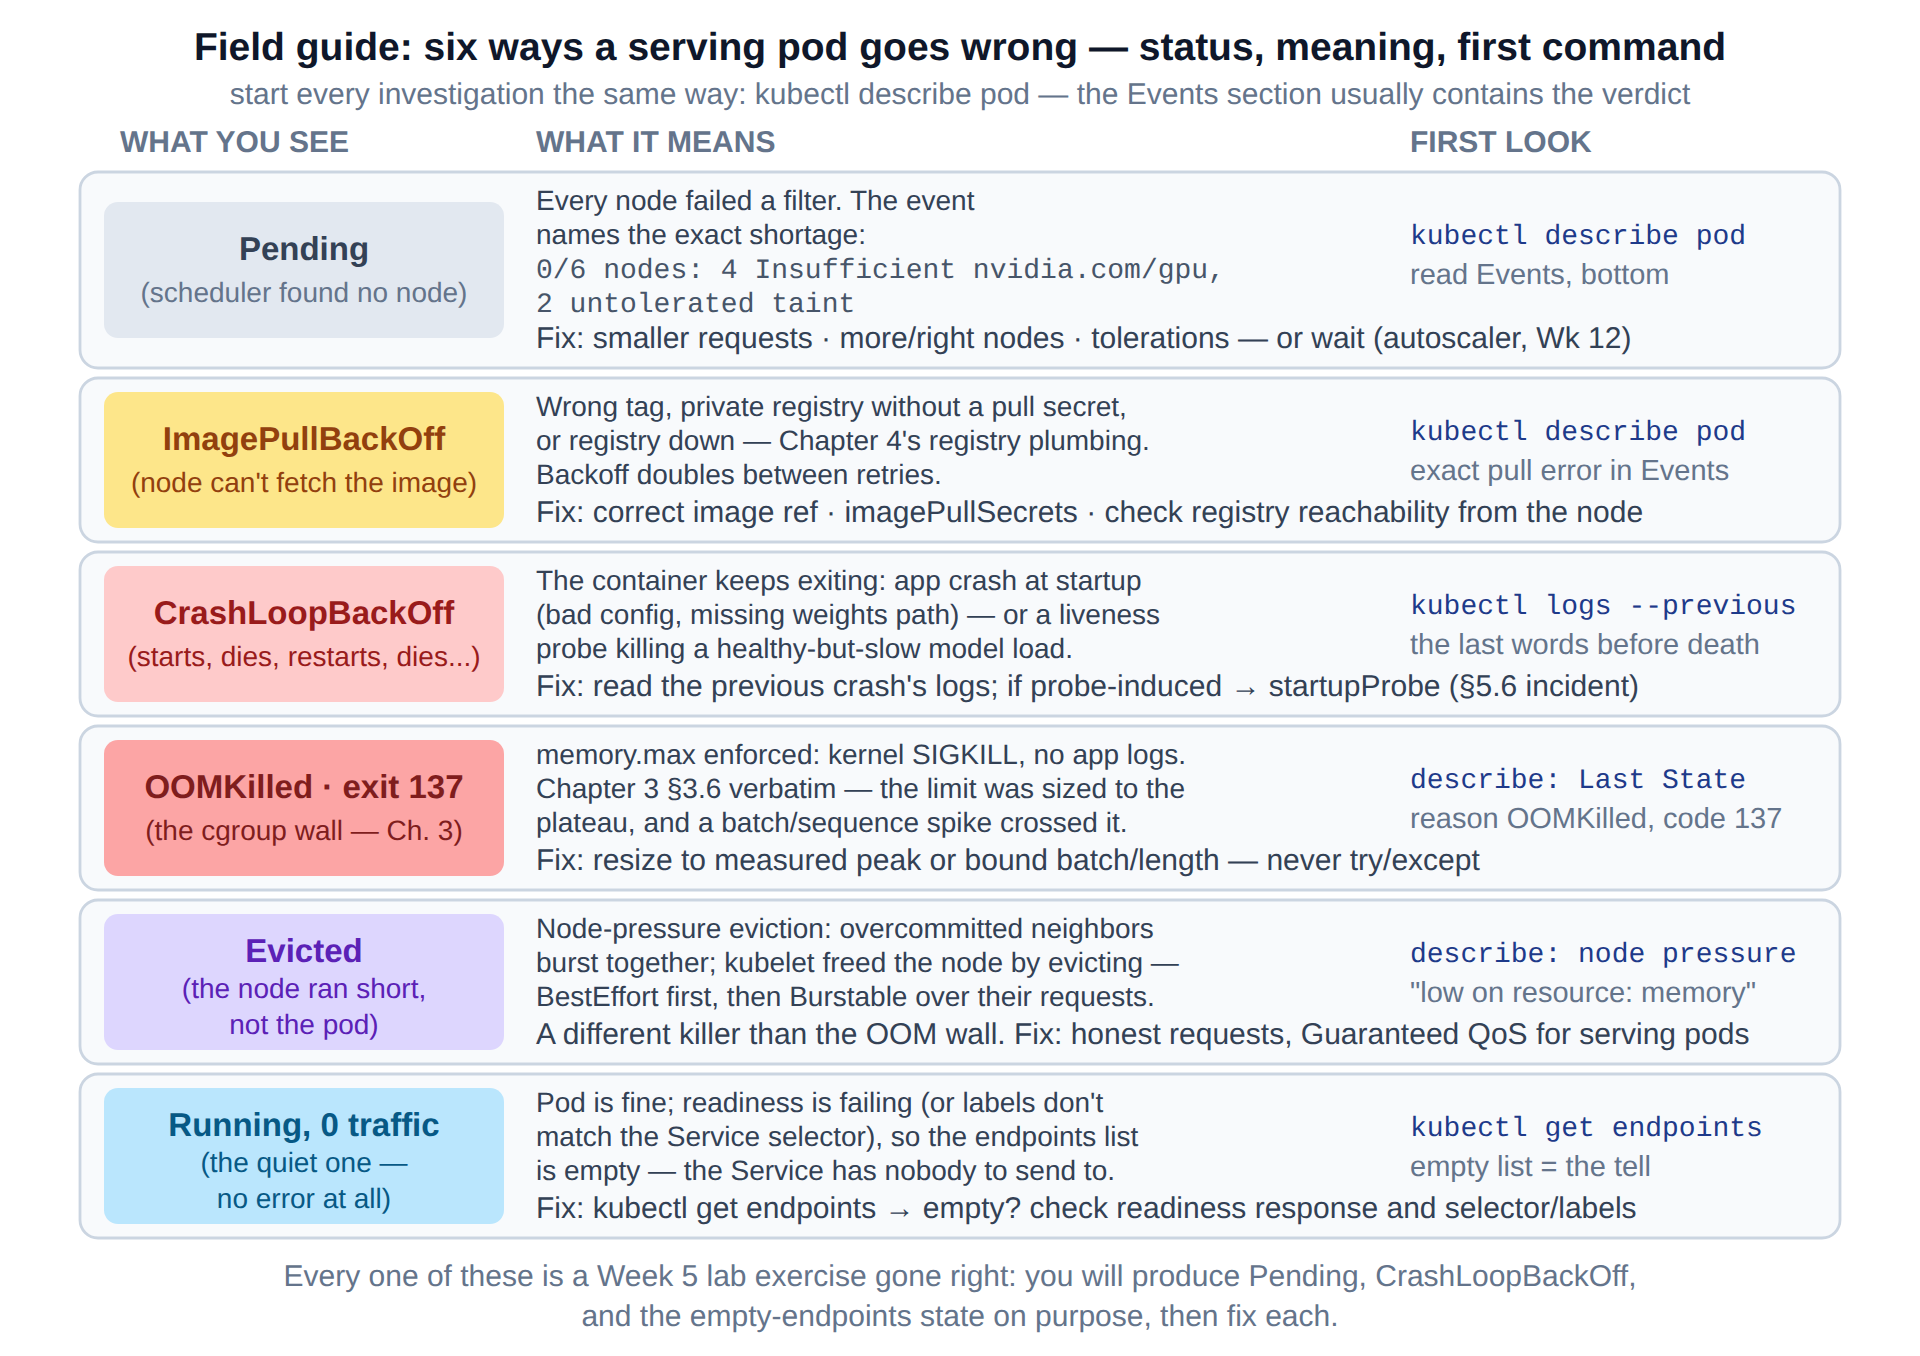
\includegraphics{figures/fig5-7_fieldguide.png}}\\[3pt]
  \figcaption{그림 5-7  여섯 가지 대표 실패 상태. 무엇이 보이고, 무엇을 뜻하며, 어디부터 살펴봐야 하는지 정리했다. 이번 주 실습에서 여섯 가지를 모두 의도적으로 재현한다.}
\end{tbbfigure}

\subsection*{사고의 전 과정: 정상 이미지에서 발생한 CrashLoopBackOff}

상황은 이렇다. 팀원이 새 모델을 로딩하는 데 \textasciitilde{}90초가 걸리는 \code{model-server:v9}를 배포했다. \code{docker run}에서는 잘 동작했다. 하지만 startupProbe는 설정하지 않고 성급한 livenessProbe를 그대로 둔 Deployment를 클러스터에서 실행하자 다음 결과가 나온다.

\begin{terminalbox}
\begin{Verbatim}[breaklines=true,breakanywhere=true,fontsize=\small,formatcom=\color{tbbtermfg},codes=\tbbcodeactive]
$ kubectl get pods
NAME                            READY   STATUS             RESTARTS   AGE
model-server-59f6c9d8b7-qv4tn   0/1     CrashLoopBackOff   5          8m
# five restarts in eight minutes. First reflex: describe, read Events.
$ kubectl describe pod model-server-59f6c9d8b7-qv4tn
...
Events:
  Warning  Unhealthy  Liveness probe failed: Get "http://10.244.1.61:8000
           /healthz": context deadline exceeded
  Normal   Killing    Container server failed liveness probe, will be
           restarted
  Normal   Pulled     Container image already present on machine
  Normal   Started    Started container server
# the kubelet is the killer - and it says so. Second reflex:
$ kubectl logs model-server-59f6c9d8b7-qv4tn --previous | tail -3
INFO  loading weights shard 5/8 ...
INFO  loading weights shard 6/8 ...
INFO  loading weights shard 7/8 ...
\end{Verbatim}
\end{terminalbox}
\figcaption{터미널 기록 5-9  포렌식 연결 고리. CrashLoopBackOff → describe가 활성 상태 프로브를 처형자로 지목 → logs --previous에는 느리게 로딩했을 뿐인 프로세스가 보인다. 잘못을 저지른 것은 아무것도 없으므로 어디에도 오류는 나타나지 않는다.}

제3장에서 OOM 연결 고리를 분석한 방식으로 읽어 보자. \textbf{상태}는 컨테이너가 계속 죽는다고 말한다. \code{CrashLoopBackOff}는 원인이 아니라 재시작 사이의 대기 시간을 두 배씩 늘리는 재시작 \textit{정책}이다. \textbf{이벤트}는 처형자를 지목한다. 단일 스레드로 가중치를 읽느라 서버가 답할 수 없을 때 응답을 요구한 활성 상태 프로브를 대신해 kubelet이 죽였다. \textbf{이전 로그}는 비행 기록 장치다. 일반 \code{logs}는 막 재시작한 \textit{현재} 시도를 보여 주지만 이전 로그는 오류 하나 없이 로딩 도중에 끝난다. 종료하고, 다시 로딩하고, 다시 종료한다. 재시작할 때마다 전체 로딩 비용을 다시 치르고(제3장의 재시작 루프 경제학), 파드는 한 번도 Ready가 되지 못했다. 해결책은 최악의 로딩 시간을 포괄하는 예산을 둔 startupProbe, 즉 터미널 기록 5-3의 구절이다. 적용하면 같은 이미지가 조용히 90초를 보낸 뒤 Ready가 된다. 이 사고보다 오래 남을 일반 교훈이 있다. \textbf{Kubernetes에서는 플랫폼 자체도 실패 원인 가운데 하나다.} 프로브, 상한, 퇴거는 정상 프로세스를 죽일 수 있으며, 증거는 애플리케이션 로그가 아니라 이벤트에 남는다.

\subsection*{Pending: 스케줄러가 풀이 과정을 보여 준다}

\begin{terminalbox}
\begin{Verbatim}[breaklines=true,breakanywhere=true,fontsize=\small,formatcom=\color{tbbtermfg},codes=\tbbcodeactive]
$ kubectl get pods
NAME                            READY   STATUS    RESTARTS   AGE
llm-server-7b9d5f4c66-x2jkp     0/1     Pending   0          3m
$ kubectl describe pod llm-server-7b9d5f4c66-x2jkp | tail -4
Events:
  Warning  FailedScheduling  0/6 nodes are available:
    4 Insufficient nvidia.com/gpu,
    2 node(s) had untolerated taint {team: batch}.
\end{Verbatim}
\end{terminalbox}
\figcaption{터미널 기록 5-10  Pending은 스케줄러가 필터 보고서를 게시한 상태다(§5.5). 노드 여섯 개가 각각 어떤 필터에서 실패했는지 정확히 보여 준다. 파드에는 아무 문제가 없고, 클러스터가 파드의 제약 조건을 충족하지 못할 뿐이다.}

Pending은 시스템에서 가장 충실하게 스스로 설명하는 상태다. §5.5의 필터 단계가 실패 집계를 이벤트에 그대로 기록하기 때문이다. \textit{"각 노드가 탈락한 이유는 다음과 같다"}라고 읽으면 된다. 해결책은 단계적으로 나뉜다. requests를 줄이고(정말 GPU 4개가 필요한가?), 용량을 비우거나 추가하고(12주 차 오토스케일러가 바로 이 일을 자동화한다), 주소 지정 문제(톨러레이션과 레이블)를 고친다. 해결책이 아닌 것도 하나 기억하자. 파드를 삭제하고 다시 만들면 같은 클러스터에 같은 필터를 다시 실행하므로 또 Pending이 된다. 증상이 아니라 제약 조건을 고쳐야 한다.

\subsection*{나머지 네 가지 상태}

\begin{tbbitemize}
  \item \textbf{ImagePullBackOff} — 노드가 이미지를 가져올 수 없다. 태그가 틀렸거나, 비공개 레지스트리에 필요한 \code{imagePullSecrets}가 없거나, 노드에서 레지스트리에 접근할 수 없는 경우다. 제4장의 레지스트리 배관 문제이며, \code{describe} events에 원본 pull 오류가 들어 있다. (미묘한 서빙 변형도 있다. tag는 존재하지만 이미지 크기가 8 GB이고 노드 디스크가 가득 찬 경우로, 이벤트가 그대로 알려 준다.)
  \item \textbf{OOMKilled / exit 137} — 제3장 §3.6의 상황을 플랫폼이 다시 보여 준다. \code{describe}에는 \code{Last State: Terminated, Reason: OOMKilled, Exit Code: 137}이 나타난다. Kubernetes에는 한 가지 변형이 있다. \code{restartPolicy}가 \textit{같은} limit로 컨테이너를 되살리므로, 너무 작은 limit는 매번 모델 로딩 콜드 스타트 비용을 치르는 충돌 루프가 된다. §3.6의 순진한 정책에 관성이 붙은 셈이다. 해결 방법은 똑같다. 측정한 최댓값에 맞게 크기를 조정하거나 변동 부분을 제한해야 하며, try/except로 처리해서는 안 된다.
  \item \textbf{Evicted} — \textit{노드}의 자원이 부족해졌다(표 5-2). 상태는 \code{Evicted}, 메시지는 "노드의 메모리 리소스가 부족함"으로 나온다. 파드는 잘못이 없었을 수도 있으며, 희생 대상은 QoS가 결정했다. 퇴거가 반복되면 노드 어딘가의 requests가 정직하지 않다는 뜻이다. 네임스페이스를 감사하고 서빙 파드를 Guaranteed로 옮긴다.
  \item \textbf{실행 중이지만 라우팅되지 않음} — 조용한 상태이자 목록에서 어디에도 오류가 없는 유일한 상태다. 파드가 실행되고 활성 상태 검사를 통과하지만 준비 상태가 끝내 true가 되지 않거나 레이블이 Service 셀렉터와 일치하지 않는다. 따라서 \textbf{엔드포인트 목록이 비고} Service는 트래픽을 보낼 곳이 없다. 클라이언트에는 연결 오류가 발생하지만 모든 파드 대시보드는 초록색이다. 이를 드러내는 명령은 \code{kubectl get endpoints model-svc} 하나다. 저자의 경험상 이 명령을 확인하는 반사 행동이 이 장에서 얻을 수 있는 가장 가치 있는 습관이다.
\end{tbbitemize}

\begin{calloutbox}{tbbpurple}{tbbpurplefill}
{\normalsize\bfseries\color{tbbpurple}다섯 가지 반사 행동(모니터에 붙여 두자)}\par\vspace{3pt}
\begin{tbbitemize}
  \item \code{kubectl describe pod <p>} — 언제나 가장 먼저 실행한다. Events에 판결문이 있다(프로브, 스케줄링, pull, OOM, 퇴거).
  \item \code{kubectl logs <p> --previous} — 비행 기록 장치다. 새 시도가 아니라 죽은 시도가 남긴 마지막 말을 보여 준다.
  \item \code{kubectl get endpoints <svc>} — 대시보드는 초록색인데 아무 응답이 없다면, 반증될 때까지 엔드포인트가 비었다고 본다.
  \item \code{kubectl exec -it <p> -- sh} — 내부로 들어가(제3장에서 이것이 setns라고 배웠다) /ready를 직접 시험하고 환경 변수와 경로를 확인한다.
  \item \code{kubectl port-forward pod/\allowbreak <p> 8000:8000} — Service를 우회해 특정 파드 하나와 통신함으로써 "파드 고장"과 "라우팅 고장"을 구분한다.
\end{tbbitemize}
\end{calloutbox}

\vspace{3.0pt}

\begin{calloutbox}{tbbpurple}{tbbpurplefill}
{\normalsize\bfseries\color{tbbpurple}생각해 보기}\par\vspace{3pt}
\begin{tbbitemize}
  \item 컨테이너가 CrashLoopBackOff를 보이고 logs --previous는 오류 없이 끝나며 exit code는 137이다. 서로 다른 두 처형자가 137을 만든다(제3장의 SIGKILL 계산). 둘을 말하고, 구별할 수 있는 정확한 describe 필드를 제시하자.
  \item 팀의 readinessProbe가 데이터베이스 의존성을 검사한다. 데이터베이스가 30초 동안 잠깐 멈추자 모든 파드가 동시에 준비되지 않은 상태가 되고 → 엔드포인트가 비며 → 캐시된 응답을 제공할 수 있었던 서비스까지 완전히 중단된다. 준비 상태 프로브(readiness probe)에서 의존성을 검사하는 방식의 장단점을 논하고 절충안을 제안하자.
  \item "모델 서버는 정상이고 Service 셀렉터가 잘못되었다"는 사실을 1분 안에 증명할 명령 순서를 설계하자. (port-forward와 get endpoints가 유용하다.)
\end{tbbitemize}
\end{calloutbox}

\section{실습: 모델 서버 오케스트레이션}

이번 주 실습에서는 제4장의 이미지를 \code{docker run}에서 관리형 플릿으로 승격한 뒤, §5.6의 모든 방식으로 의도적으로 망가뜨린다. 모든 과정은 노트북에서 실행된다. \code{minikube start --cpus 4 --memory 8g}를 사용하며 kind도 똑같이 동작한다. 이미지는 강의 레지스트리에서 제공하고, 공개 대체 태그는 유인물에 있다. 이번 주에는 클라우드 비용이 필요 없다. §5.5의 GPU 터미널 기록은 시연 전용이며, 이미 크레딧이 있는 팀을 위해 관리형 클러스터에서 재현하는 선택 부록을 제공한다. \code{kubectl create namespace ml}로 만든 네임스페이스 안에서 작업한다.

\subsection*{파트 A — 배포하고 노출한 뒤 루프를 신뢰하기}

터미널 기록 5-3의 Deployment와 터미널 기록 5-6의 Service를 적용한다(minikube에서는 NodePort 유형). \code{get pods -o wide}로 플릿을 확인한 뒤, \textbf{자기 플릿에서 터미널 기록 5-1의 실험을 다시 실행}한다. curl 루프 도중 파드를 삭제하고 조정 과정을 기록한다. 이어서 터미널에서 Service에 초당 요청 하나를 보내는 curl 루프를 실행한 채 \code{:v8}로 롤링 업데이트한다. 제출물의 핵심 장면은 전체 롤아웃 동안의 루프 출력이다. 준비 상태가 속도를 제어하고 제3장의 SIGTERM 핸들러가 기존 파드의 처리 중인 요청을 비우므로 \textbf{실패한 요청은 0개}여야 한다. (그런 다음 의도적으로 망가뜨린다. readinessProbe를 제거하고 \code{:v9-slow}로 롤아웃해 같은 curl 루프에서 오류가 나는 모습을 확인한다. 준비 상태의 효과를 증명하는 음성 대조군이다.)

\subsection*{파트 B — 직접 검증하는 변환 관계}

터미널 기록 5-7을 직접 재현한다. \code{minikube ssh}로 접속해 \code{/\allowbreak sys/\allowbreak fs/\allowbreak cgroup/\allowbreak kubepods.slice/\allowbreak } 아래의 cgroup 트리를 따라가고, YAML의 숫자가 \code{memory.max}와 \code{cpu.max}에 들어 있는 모습을 캡처한다. 자기 터미널에서 이 장의 핵심을 증명하는 것이다. 그런 다음 OOM을 재현한다. 표준 모델에 \code{limits.memory: 256Mi}를 설정해 적용하고, Kubernetes식 증거 연결 고리를 수집한다. \code{describe}의 \code{OOMKilled /\allowbreak  137}과 함께 충돌 루프가 매번 모델 로딩 콜드 스타트 비용을 치르면서 재시작 횟수가 증가하는 모습을 담는다. 정직한 상한으로 복구하고, §3.6의 어휘를 사용해 전후 차이를 보고서에 기록한다.

\subsection*{파트 C — 망가뜨리고, 진단하고, 고치기}

세 가지 사고를 재현한다. 각 사고는 해결책을 적용하고 어떤 절에서 이를 예측했는지 한 문장으로 밝히며 끝낸다. \textbf{(1) Pending:} GPU가 없는 minikube에서 \code{nvidia.com/\allowbreak gpu: 1}을 요청한다. FailedScheduling 이벤트를 캡처하고 필터 보고서를 소리 내어 읽은 뒤(§5.5), 요청을 제거해 고친다. \textbf{(2) 프로브 사고:} 환경 변수 \code{SLOW\_LOAD=90}을 설정해 강의 이미지가 느린 모델 로딩을 모의하게 하고, startupProbe를 삭제하며, 활성 상태 프로브를 \code{periodSeconds: 5, failureThreshold: 2}로 강화한다. 터미널 기록 5-9의 전체 포렌식 연결 고리인 상태, 이벤트, \code{logs --previous}를 재현한다. startupProbe 설정으로 고치고 같은 이미지가 Ready가 되는 모습을 보여 준다. \textbf{(3) 조용한 실패:} 준비 상태 경로를 서버가 제공하지 않는 오타 \code{/\allowbreak readyz}로 바꾼다. Running 상태 파드, 정상인 활성 상태 검사, 비어 있는 \code{get endpoints}, 실패하는 클라이언트 curl 요청을 관찰한다. 수정한 뒤 엔드포인트가 다시 채워지는 모습을 확인한다.

\begin{calloutbox}{tbbpurple}{tbbpurplefill}
{\normalsize\bfseries\color{tbbpurple}실습 체크리스트}\par\vspace{3pt}
\begin{tbbitemize}
  \item 파트 A 결과물: 플릿의 \code{get pods -o wide} · 삭제와 조정 캡처 · 롤링 업데이트 내내 중단 없이 실행된 curl 루프 · 음성 대조군(준비 상태 검사 없음 → 오류).
  \item 파트 B 결과물: YAML과 일치하는 노드 쪽 \code{memory.max}와 \code{cpu.max} · 재시작 횟수를 포함한 OOMKilled describe 블록 · 복원한 설정.
  \item 파트 C 결과물: FailedScheduling 필터 보고서 · 터미널 기록 5-9 재현(이벤트 + logs --previous)과 수정 후 Ready 상태 · 비어 있는 엔드포인트라는 징후와 다시 채워진 모습.
  \item 보고서: 한 페이지, 관찰 세 가지, 각각 관련 절을 명시(예: "활성 상태 프로브 종료는 애플리케이션 로그를 남기지 않았다 — §5.6의 실패 원인으로서의 플랫폼").
  \item 정리: \code{kubectl delete namespace ml}; \code{minikube stop}. (이번 주에는 클라우드 비용이 없지만 습관은 유지한다.)
\end{tbbitemize}
\end{calloutbox}

\vspace{3.0pt}

\begin{calloutbox}{tbbpurple}{tbbpurplefill}
{\normalsize\bfseries\color{tbbpurple}생각해 보기}\par\vspace{3pt}
\begin{tbbitemize}
  \item 파트 A의 롤링 업데이트 동안 curl 루프는 한 번도 실패하지 않았다. 준비 상태 관문과 엔드포인트 갱신부터 제3장의 SIGTERM 핸들러까지 협력해야 했던 모든 메커니즘을 열거하고, 어느 하나를 제거했을 때 가장 손쉽게 보장이 깨지는지 찾자.
  \item minikube는 노드가 하나다. 실제 노드 다섯 개 클러스터라면 달라질 실습 동작 세 가지와, 단일 노드 클러스터에서는 제대로 재현할 수 없는 §5.6의 상태 하나를 말해 보자.
\end{tbbitemize}
\end{calloutbox}

\namedsection{요약}{열 가지로 정리한 이 장}

\qitem{1}{\textbf{Kubernetes는 조정 루프다.} 원하는 상태는 etcd에 있고, 컨트롤러는 영원히 관찰하고 차이를 찾고 동작한다. 명사를 선언하면 동사가 자연스럽게 나타난다. 삭제된 파드는 누군가 처리할 이벤트가 아니라 편차이며, 편차는 교정된다.}

\qitem{2}{\textbf{선언형 불변 조건은 시간이 지나도 효력을 잃지 않으므로 명령형 지시보다 강하다.} 노드 장애, 실수로 누른 삭제, 배포는 루프의 관점에서 모두 같다. 오토스케일링(12주 차)과 CI/CD(13주 차)는 원하는 상태를 작성하는 주체가 하나씩 더 늘어나는 것뿐이다.}

\qitem{3}{\textbf{구조는 자기주장이 있는 데이터베이스다.} API 서버(유일한 출입구), etcd(유일한 상태), 스케줄러(중매자), 컨트롤러 매니저(루프), kubelet(손발), kube-proxy(NAT)로 구성된다. 구성 요소끼리는 직접 호출하지 않고 모든 통신은 API 서버를 감시하는 방식로 이루어진다. 그래서 어느 한 구성 요소가 죽어도 시스템 전체가 중단되지 않는다.}

\qitem{4}{\textbf{Kubernetes라는 이름의 무언가가 컨테이너를 실행하는 것이 아니다.} 연결 고리는 apply → 객체 생성 → 스케줄러 바인딩 → kubelet → CRI → containerd → runc → 제3장의 네임스페이스와 cgroup이다. 마지막에 memory.max를 작성하는 대필자는 kubelet이다.}

\qitem{5}{\textbf{파드는 스케줄링과 공유의 단위다.} 컨테이너는 pause 컨테이너의 NET 네임스페이스(하나의 IP, localhost로 연결된 사이드카)에 합류하고 볼륨을 공유하며, MNT와 PID는 각자 분리된다. 파드는 언젠가 사라지고 레이블로 주소를 지정하므로 IP를 직접 대상으로 삼아서는 안 된다. 이 모든 것이 가정하는 워크로드 형태는 \textbf{마이크로서비스}다. 서비스마다 기능 하나를 두고 코드 복잡성을 운영 복잡성과 맞바꾼다. 세 축은 이 절충 관계의 입문 키트이며, 마이크로서비스 하나 = Deployment 하나 + Service 하나다.}

\qitem{6}{\textbf{프로브는 서로 다른 세 질문을 던진다.} 시작 프로브("부팅을 마쳤는가?")는 모델 로딩을 보호하고, 준비 상태 프로브("트래픽을 보내도 되는가?")는 Service 엔드포인트와 롤아웃 속도를 제어하며, 활성 상태 프로브("살아 있기는 한가?")는 재시작한다. 로딩에 90초가 걸리는 모델에서 활성 상태와 준비 상태를 혼동하면 정상 이미지가 영원히 충돌 루프를 돈다.}

\qitem{7}{\textbf{Deployment는 기계적인 방식으로 무중단 롤아웃을 만든다.} 템플릿 버전마다 ReplicaSet 하나를 두고, maxSurge/maxUnavailable로 속도를 조절하며, 준비 상태를 관문으로 사용하고, 롤백할 때는 이전 대상을 다시 가리킨다. Terminating 파드마다 제3장의 SIGTERM 과정이 되풀이된다. 처리 중인 요청을 비우는 일은 핸들러가 하고 Kubernetes는 그 작업을 스케줄링할 뿐이다.}

\qitem{8}{\textbf{requests는 스케줄러의 산술 값이고 limits는 cgroup의 벽이다.} requests.cpu는 유연하고 작업 보존적인 cpu.weight의 바탕도 된다. limits는 cpu.max(버스트 스로틀링 — §3.3에서 만든 p99)와 memory.max(§3.6의 OOM 벽)가 된다. requests와 limits 사이의 간격은 의도적인 오버커밋이다. 가정이 틀리면 kubelet이 퇴거를 수행하며, 이는 Evicted 대 OOMKilled/137이라는 서로 다른 징후를 보이는 두 번째 처형자다. QoS 클래스(Guaranteed / Burstable / BestEffort)는 oom\_score\_adj를 설정하며, 서빙 파드는 Guaranteed로 실행한다.}

\qitem{9}{\textbf{GPU는 정수 단위 확장 리소스로 스케줄링된다. 일부만 요청할 수 없고 오버커밋도 없으며 requests = limits다. GPU 공유를 중재할 cgroup 컨트롤러가 없기 때문이다(제3장에서 비어 있던 부분).} 테인트는 밀어내고 어피니티는 방향을 정하며 디바이스 플러그인은 리소스를 알리고 할당한다. GPU 플릿은 빈 패킹해야 한다. 단편화는 비용이 붙은 Pending이고 고립된 GPU는 유휴 상태로도 비용이 청구된다. 일부만 나누어 쓰는 방식은 제2장의 MIG/시간 분할에서 온다(12주 차).}

\qitem{10}{\textbf{여섯 가지 상태가 거의 모든 서빙 사고를 포괄한다.} Pending(필터 보고서 확인), ImagePullBackOff(제4장의 배관), CrashLoopBackOff(애플리케이션 충돌 또는 프로브 종료 — logs --previous), OOMKilled/137(제3장과 동일), Evicted(노드 압박), 실행 중이지만 라우팅되지 않음(빈 엔드포인트 — 조용한 실패)다. describe → 이벤트가 진단의 출입구이며 플랫폼 자체도 실패 원인 가운데 하나다.}

\namedsection{연습문제}{}

\subsection*{A. 객관식}

\qitem{1}{레플리카가 세 개인 Deployment에서 파드 하나를 삭제했다. 어떤 메커니즘으로 무슨 일이 일어나는가?}

\begin{tbboptions}
  \item ① 아무 일도 일어나지 않는다. 파드는 다음 배포 때만 다시 생성된다.
  \item ② restartPolicy가 Always이므로 kubelet이 같은 파드를 재시작한다.
  \item ③ ReplicaSet 컨트롤러가 원하는 수 3 ≠ 실제 수 2를 관찰하고 새 파드를 만든다(새 이름, 경우에 따라 새 노드).
  \item ④ kube-proxy가 Service의 엔드포인트 캐시에서 파드를 다시 만든다.
\end{tbboptions}

\qitem{2}{limits.memory: 1.75Gi를 노드의 memory.max 파일로 바꾸는 구성 요소는 무엇인가?}

\begin{tbboptions}
  \item ① 매니페스트를 검증할 때의 API 서버
  \item ② 바인딩 시점의 스케줄러
  \item ③ 저장소 훅을 거치는 etcd
  \item ④ CRI를 통해 컨테이너 런타임을 구동하는 노드의 kubelet
\end{tbboptions}

\qitem{3}{requests와 limits에 관한 설명으로 옳은 것은?}

\begin{tbboptions}
  \item ① requests는 cpu.max가 강제하고 limits는 권고값이다.
  \item ② requests는 스케줄러의 배치와 cpu.weight에 쓰이고, limits는 런타임에 강제되는 cgroup 벽이 된다.
  \item ③ 둘 다 똑같이 강제되며 requests는 단지 최솟값이다.
  \item ④ limits는 GPU에만 영향을 준다.
\end{tbboptions}

\qitem{4}{파드가 Running이고 liveness도 통과하지만 클라이언트가 Service를 통해 연결 오류를 겪는다. 가장 먼저 확인할 가치가 큰 항목은?}

\begin{tbboptions}
  \item ① kubectl logs — 스택 추적를 찾는다.
  \item ② Deployment를 재시작한다.
  \item ③ kubectl get 엔드포인트 — 목록이 비었다면 준비 상태 또는 셀렉터가 문제다.
  \item ④ 노드를 재부팅한다.
\end{tbboptions}

\qitem{5}{컨테이너가 메모리에서만 requests = limits로 설정했고 CPU request는 CPU limit보다 작다. 이 컨테이너의 QoS 클래스는?}

\begin{tbboptions}
  \item ① Guaranteed — 중요한 것은 메모리다.
  \item ② Burstable — Guaranteed가 되려면 모든 컨테이너의 CPU와 메모리에서 requests = limits여야 한다.
  \item ③ BestEffort — 클래스는 CPU가 결정한다.
  \item ④ 노드의 allocatable에 따라 달라진다.
\end{tbboptions}

\qitem{6}{1-GPU 파드가 계속 Pending에 머문다. describe에는 "노드 0/6개를 사용할 수 없음: 4개는 nvidia.com/gpu 부족, 2개는 허용되지 않은 테인트 \{nvidia.com/gpu: present\}가 있음."라고 나온다. 실제로 노드 두 개에는 여유 GPU가 있다. 올바른 해결책은?}

\begin{tbboptions}
  \item ① 파드의 CPU requests를 늘려 다른 파드보다 높은 값을 제시한다.
  \item ② 파드에 일치하는 톨러레이션을 추가해 테인트가 붙은 GPU 노드 두 개가 필터링을 통과하게 한다.
  \item ③ 더 쉽게 들어가도록 nvidia.com/gpu: 0.5로 설정한다.
  \item ④ 파드를 삭제하고 다시 만들어 스케줄링을 다시 실행한다.
\end{tbboptions}

\subsection*{B. 단답형}

\qitem{1}{레플리카가 3개인 새 Deployment에 kubectl apply를 실행한 순간부터 컨테이너가 실행될 때까지를 다섯 단계로 추적하고, 단계마다 담당 구성 요소를 밝히자.}

\qitem{2}{노드에서 Σ limits > allocatable은 허용되지만 Σ requests > allocatable은 불가능한 이유는 무엇인가? 오버커밋 가정이 틀렸을 때 대응하는 두 가지 안전장치도 말하자.}

\qitem{3}{모델 로딩에 최대 120초가 걸리는 서버에 적합한 프로브 설정(프로브 유형, 주기, failureThreshold)을 작성하고, 각 숫자의 근거를 한 구절씩 제시하자.}

\qitem{4}{OOMKilled와 Evicted를 비교해 각각 발동 조건, 처형자, 한 줄짜리 징후를 제시하자.}

\subsection*{C. 논술형}

\qitem{1}{"지연 시간에 민감한 서빙 파드에는 CPU limits를 절대 설정하지 말라." §3.3의 스로틀링 계산, cpu.weight의 작업 보존적 동작, Guaranteed-QoS 요구사항, 플랫폼 거버넌스의 현실을 근거로 찬반을 논하자. 강의 프로젝트의 모델 서버에 적용할 권고안을 밝히고 옹호하자.}

\qitem{2}{하나의 클러스터에서 (a) T4에서 실행되는 지연 시간에 민감한 양자화 모델, (b) A100을 원하는 야간 배치 스코어링 작업, (c) 일반 CPU 마이크로서비스를 서빙하기 위한 노드 풀, 레이블, 테인트, QoS 선택, 패킹 정책을 설계하자. 각 선택이 방지하는 실패 또는 비용 시나리오로 근거를 제시하고, 12주 차 오토스케일러가 설계에 무엇을 추가하는지 밝히자.}

\qitem{3}{"자가 복구는 근본 원인을 숨긴다. 충돌하는 파드를 조용히 교체하는 조정 루프는 사고 해결 시스템이 아니라 사고 억제 시스템이다." 모델 로딩의 재시작 루프 경제학(§3.6, §5.6), §5.6의 관측 표면, 수렴과 진단을 양립시키기 위해 성숙한 팀이 추가해야 할 것(14주 차)을 바탕으로 논하자.}

\namedsection{정답과 해설}{}

\subsection*{A. 객관식}

\qitem{1}{\textbf{③} 되살리는 것이 아니라 조정한다. ReplicaSet 조정 루프가 2 ≠ 3을 세고 새 파드(새 접미사, 새 IP, 경우에 따라 새 노드)를 만든다. ②는 파드 내부의 컨테이너 재시작과 파드 교체를 혼동했다. (§5.1)}

\qitem{2}{\textbf{④} kubelet은 손발이자 대필자다. CRI를 통해 containerd/runc를 구동하고, 이들이 cgroup 파일을 작성한다. API 서버는 저장하고 스케줄러는 배치할 뿐, 어느 쪽도 노드를 건드리지 않는다. (§5.2, §5.4)}

\qitem{3}{\textbf{②} 이 장의 핵심 비대칭이다. requests는 계획용 숫자로 런타임에 강제되지 않으며 CPU 요청량은 cpu.weight의 바탕도 된다. limits는 매 밀리초 강제되는 제3장의 cgroup 벽이다. (§5.4)}

\qitem{4}{\textbf{③} 실행 중이지만 라우팅되지 않는 상태는 조용한 실패다. 활성 상태 검사는 초록색이지만 준비 상태 검사가 실패하거나 레이블이 셀렉터와 맞지 않아 → 엔드포인트가 비고 → Service에는 보낼 대상이 없다. 잘못을 저지른 것이 없으므로 로그(①)에는 아무것도 나타나지 않는다. (§5.3, §5.6)}

\qitem{5}{\textbf{②} Guaranteed는 엄격하다. \textit{모든} 컨테이너의 \textit{두} 리소스에서 requests = limits여야 한다. 일부만 같으면 Burstable이다. 메모리만 Guaranteed처럼 설정하는 것은 흔하고 합리적인 서빙 절충안이지만 클래스 이름은 아니다. (§5.4)}

\qitem{6}{\textbf{②} 필터 보고서를 읽으면 된다. 노드 네 개에는 여유 GPU가 없고, 두 개에는 있지만 테인트가 붙었으며 파드에는 톨러레이션이 없다. 톨러레이션이 테인트가 붙은 두 노드의 문을 연다. ③은 정수만 허용되므로 불법이고, ④는 같은 필터를 다시 실행해 같은 판결을 낸다. (§5.5, §5.6)}

\subsection*{B. 단답형}

\qitem{1}{(1) API 서버가 Deployment를 검증하고 etcd에 저장한다. (2) Deployment 컨트롤러가 ReplicaSet을 만들고, ReplicaSet 컨트롤러가 nodeName이 비어 있는 Pod 객체 3개를 만든다. (3) 스케줄러가 각 파드를 필터링/점수화/바인딩해 노드에 배치한다. (4) 각 노드의 kubelet이 이미지를 가져오고 containerd → runc를 구동해 네임스페이스, cgroup, overlayfs를 만든다. (5) kubelet이 상태를 보고하고 프로브가 통과하면 엔드포인트가 파드를 받아들인다. (§5.2)}

\qitem{2}{스케줄러는 requests만 계산하므로 배치 과정에서 이를 초과 예약할 수 없다. limits는 합계가 노드 용량을 넘도록 의도적으로 허용하는 버스트 상한이다. 모두가 버스트할 수 있지만 동시에 그러는 일은 드물다는, 기능으로서의 오버커밋이다. 가정이 틀릴 때를 위한 안전장치는 컨테이너별 cgroup 벽(memory.max → OOMKilled/137)과 kubelet의 노드 압박 퇴거(QoS 순서, 상태 Evicted)다. (§5.4)}

\qitem{3}{startupProbe: httpGet /healthz, periodSeconds 5, failureThreshold ≥ 30이다. 5 × 30 = 150 s > 120 s로 최악의 로딩 시간에 여유를 더해 다른 프로브를 보류한다. readinessProbe: /ready, 주기 5, 임계값 2–3으로 트래픽을 빠르게 제어한다. livenessProbe: /healthz, 주기 10–15, 임계값 3으로 의도적으로 느긋하게 잡아 실제 교착 상태만 재시작한다. (§5.3, §5.6)}

\qitem{4}{OOMKilled: 컨테이너가 자기 memory.max를 넘었고 커널 OOM 킬러가 SIGKILL을 보낸다. 징후는 Last State: OOMKilled, exit 137(+ dmesg)이다. Evicted: 오버커밋 상태에서 노드 자원이 부족해져 kubelet이 QoS/requests 초과 사용량에 따라 희생 대상을 종료한다. 징후는 상태 Evicted, "노드의 메모리 리소스가 부족함."다. (§5.4, §5.6)}

\subsection*{C. 논술형(채점 기준)}

\qitem{1}{"limit를 설정하지 말라"는 쪽은 §3.3의 계산(30 ms 작업 → 0.2-CPU 상한에서 110–190 ms, p99 급증, 프로파일러에는 보이지 않음), cpu.weight가 자원을 낭비하지 않으면서 이미 경합의 공정성을 보장한다는 점, 유휴 여유분은 저렴한 보험이라는 점을 들어야 한다. 반대쪽은 플랫폼 규모의 폭주 방지와 비용 관리, 정직하지 않은 requests를 설정한 파드로부터 멀티테넌트 공정성을 지키는 문제, Guaranteed QoS가 limits를 요구하고 오버커밋 노드에서 Guaranteed의 OOM 보호가 중요하다는 점, 정적 CPU 매니저 고정에 정수 requests = limits가 필요하다는 점을 들어야 한다. 좋은 답은 이 긴장을 다룬 뒤 입장을 정한다. 예를 들어 측정한 최대 CPU보다 넉넉하게 requests = limits(Guaranteed)를 설정하거나, CPU limit 없이 메모리만 Guaranteed인 Burstable과 PriorityClass를 사용하고 각각의 절충 관계를 밝힌다. (§5.4)}

\qitem{2}{다음 요소를 확인한다. gpu=t4/a100 레이블이 붙은 세 노드 풀(t4-serving, a100-batch, cpu-general), 일반 CPU 작업이 들어오지 않도록 두 GPU 노드 풀에 적용한 테인트(§5.5), 톨러레이션 + gpu=t4 어피니티와 Guaranteed QoS를 적용한 모델 A 파드, 낮은 PriorityClass로 a100 노드 풀을 허용하고 CPU limits는 두지 않은 배치 작업 B, 축소와 다중 GPU 여유 공간을 위한 GPU 노드 풀의 빈 패킹(MostAllocated) 점수, 유휴 고립을 피하도록 GPU 파드에 설정한 정직한 CPU requests다. 비용 시나리오는 단편화로 인한 강제 노드 추가, CPU를 많이 쓰는 DaemonSet 뒤에 고립된 GPU, 배치 작업이 지연 시간에 민감한 파드를 선점하는 문제(우선순위 + 테인트로 방지)다. 12주 차에는 오토스케일러가 빈 패킹으로 비워진 노드를 삭제하고 배치 노드 풀을 0까지 축소한다. (§5.4–5.5)}

\qitem{3}{좋은 답은 먼저 전제의 근거를 인정한다. 90 s마다 자가 복구하는 충돌 루프의 모델 서버는 매번 콜드 스타트 지연 시간을 치르면서도 너무 작은 limit를 몇 주 동안 숨길 수 있고(§3.6의 관성), 터미널 기록 5-9의 사고는 애플리케이션 로그 증거를 전혀 남기지 않는다. 그런 다음 반론한다. 수렴이 새벽 3시의 장애를 견디게 하며, 루프는 증거를 숨기기보다 재시작 횟수, 이벤트, Last State, memory.events에 \textit{국소화}한다. 애플리케이션이 아니라 플랫폼의 표면을 보면 된다. 성숙한 운영(14주 차)은 재시작 횟수, oom\_kill 카운터, 비어 있는 엔드포인트, 멈춘 롤아웃에 경보를 건다. 즉 가용성뿐 아니라 편차 교정의 \textit{빈도}에 경보를 건다. 관측 가능성 없는 조정은 사고 억제지만, 관측 가능성과 결합하면 진단 시간을 벌어 주는 사고 \textit{완충}이라는 결론을 높이 평가한다. (§5.1, §5.6)}

\namedsection{더 읽을거리}{}

\textbf{[이번 주]} 표시가 붙은 항목은 이번 주 필독 자료다. \textbf{[N주 차]} 표시는 해당 주에 도움이 될 자료를 뜻한다.

\begin{tbbitemize}
  \item \textbf{[이번 주] Kubernetes 문서: Concepts → "Pods", "Deployments", "Service"} — §5.3의 바탕이 되는 공식 설명이다. 작업 페이지가 아니라 Concepts 페이지를 읽자. 개념 문서는 튜토리얼이 생략하는 \textit{이유}를 설명한다.
  \item \textbf{[이번 주] Kubernetes 문서: "Pod Lifecycle"} (프로브 포함) — §5.3의 세 질문, 컨테이너 상태, 재시작 백오프에 관한 권위 있는 자료다. §5.6의 CrashLoopBackOff 메커니즘도 모두 여기에 있다.
  \item \textbf{[이번 주] Kubernetes 문서: "Resource Management for Pods and Containers" + "Configure Quality of Service for Pods"} — §5.4의 1차 자료다. requests와 limits, allocatable, QoS 클래스, 그리고 노드 문서에 나오는 노드 압박 퇴거 순서를 다룬다.
  \item \textbf{Kelsey Hightower, "Kubernetes the Hard Way" (GitHub)} — 설치 도구 없이 클러스터를 한 번 만들어 보면 §5.2의 구조가 더 이상 그림에 머물지 않는다. 비 오는 주말에 평생 한 번만 해 보자. 그 정신 모형은 경력 내내 남는다.
  \item \textbf{Marko Lukša, "Kubernetes in Action" (2nd ed., Manning)} — 책 한 권 분량으로 다룬 자료 가운데 가장 좋다. Pod, Deployment, Service, 리소스 관리 장은 더 넓은 API 표면을 다루면서도 §5.3–5.4와 일대일로 대응한다.
  \item \textbf{Verma et al., "Large-scale cluster management at Google with Borg" (EuroSys 2015)} — 선언형 작업, 조정, 빈 패킹, §5.5가 물려받은 사용률 경제학의 기원을 보여 준다. §5(utilization)를 제1장의 비용 관점으로 읽자.
  \item \textbf{[6주 차] Kubernetes 문서: "Ingress" 및 클라우드 공급업체 로드 밸런서 문서} — 6주 차에 Service 앞에 추가할 계층(API 게이트웨이, TLS, 라우팅)을 다룬다.
  \item \textbf{[12주 차] NVIDIA GPU Operator 및 디바이스 플러그인 문서(시간 분할, MIG 전략); Kubernetes Cluster Autoscaler FAQ; HPA/KEDA 문서} — §5.5의 운영상 후속 내용인 분할 GPU, Pending에 따른 확장, 빈 패킹으로 비운 노드의 축소, 이벤트 기반 오토스케일링을 다룬다.
  \item \textbf{[13주 차] Argo Rollouts 문서(카나리, 블루-그린)} — 13주 차에 점진적 전달(progressive delivery)과 자동 분석을 추가하면 Deployment의 롤링 업데이트가 어떤 형태로 발전하는지 보여 준다.
\end{tbbitemize}

\vspace{5.0pt}

\begin{calloutbox}{tbbblue}{tbbbluefill}
{\normalsize\bfseries\color{tbbblue}다음 장 — 제6장: 스토리지와 네트워킹}\par\vspace{3pt}
이제 모델 서버는 안정적인 이름을 가진 플릿으로 실행된다. 하지만 가중치는 여전히 이미지에 구워 넣은 상태이고(제3장에서 경고했다), Service도 여전히 클러스터 내부 배관에 머문다. 다음 주에는 서빙의 골격을 완성한다. \textbf{블록 스토리지(block storage)와 객체 스토리지}의 차이와 모델 가중치를 객체 스토어(object store)에 보관하는 이유, S3 호환 스토리지에 가중치와 데이터셋을 두고 시작할 때 로딩하며 이미지와 독립적으로 버전을 관리하는 \textbf{모델 저장소 패턴}(6주 차 실습에서 바로 이 경로를 만들고 13주 차 레지스트리 이야기의 바탕이 된다), Service 앞의 출입구인 \textbf{로드 밸런서와 API 게이트웨이}, 값비싼 GPU 플릿을 공개 인터넷에서 격리하는 데 필요한 \textbf{VPC와 보안 그룹(security group)} 기본 지식을 다룬다. 6주 차가 끝나면 강의의 인프라 절반이 완성되고, 파트 2에서는 그 위에서 모델 서빙을 시작한다.
\end{calloutbox}
